\resetgraphicspath
\appendtographicspath{{./Chapter 1/figures/} }
\appendtographicspath{{./Chapter 1/figures/Procedural/} }
\appendtographicspath{{./Chapter 1/islands/} }
\appendtographicspath{{./Chapter 1/Results/} }
\appendtographicspath{{./Chapter 1/Results/Procedural/} }

\chapter{Automatic generation of coral reef islands}
\label{chap:coral-island}
\teaser{
\autofitgraphics[]{Teaser1.png, Teaser2.png, Teaser3.png}
\centering
\caption{Given a free hand-drawn sketch of the different regions of an island (bottom inset of each example), our method generates a corresponding height field using neural networks. Subsidence (gradual sinking of land) is controlled by the user in the luminosity channel of the input. These examples show the gradual subsidence of the same island over time.}
\label{fig:teaser_cGAN}
}

\abstract
In this chapter, we propose a procedural method for generating single volcanic islands with coral reefs using user sketching from two projections: a top view, which defines the island's shape, and a profile view, which outlines its elevation. These projections, commonly used in geological and remote sensing domains, are complemented by a user-defined wind field, applied as a distortion field to deform the island's shape, mimicking the effects of wind and waves in the long term and enabling finer user control. We then model the growth of coral on the island and its surroundings to construct the reef following biological observations. Based on these inputs, our method generates a height field of the island. Our method creates a large variety of island models to compose a dataset used for training a conditional Generative Adversarial Network (cGAN). By applying data augmentation, the cGAN allows for even greater variety in the generated islands, providing users with greater freedom and intuitive controls over the shape and structure of the final output.
\pagebreak

\minitoc

\section{Introduction}
\label{sec:coral-island-introduction}

\begin{figure}[H]
\autofitgraphics[]{Kauai_island.png, Tuvuca_island.png, Mascarene_island.png, Cocos_island.png}
\caption{Kauai Island, Tuvuca Island, Mascarene Island, and Cocos Island (from left to right) are islands formed through an identical geological process; however, their shapes vary greatly, from a full island with fringing coral reef (leftmost) to a complete atoll (rightmost).}
\label{fig:coral-island-island-examples}
\end{figure}

Charles Darwin's subsidence theory, developed from his observations in \citep{Darwin1842}, remains one of the most widely accepted explanations for the formation of coral reef islands such as those presented in \cref{fig:coral-island-island-examples}. His theory states that they are formed through a dynamic interplay of volcanic activity, coral growth, and long-term geological processes. These islands begin as volcanic landmasses, created when magma from the Earth's mantle erupts through the ocean floor and builds up layers of volcanic rock, eventually rising above sea level (\cref{fig:coral-island-island-growth}). In tropical waters, these volcanic islands create ideal conditions for coral reefs to develop. Corals, thriving in the shallow, sunlit waters around the island, initially form fringing reefs attached to the island's coastline.

\begin{figure}[H]
\centering
\includegraphics[width = \linewidth]{other_images/Drawings/Volcano.jpg}
\caption{Volcanic islands rise above hotspots. The rise of magma from the hotspot forms a seamount. Consecutive eruptions from the volcano grow the seamount until the peak emerges above sea level. The ground above and close to sea level is affected by hydraulic, aeolian, and coastal erosion.}
\label{fig:coral-island-island-growth}
\end{figure}

As time passes, the volcanic island undergoes subsidence, a slow sinking process caused by the cooling and contraction of the Earth's crust beneath the island. In response to this subsidence, corals continue to grow upwards, maintaining their position within the photic zone, where sunlight supports their survival. This upward growth leads to the formation of barrier reefs, which become separated from the island by a lagoon as the island sinks further.

Eventually, the volcanic island may submerge completely beneath the ocean's surface, leaving only the coral structure visible above water. This process results in the formation of atolls, which are ring-shaped reefs encircling a central lagoon. Over geological time, the physical structure of the island evolves from a prominent volcanic peak to a coral-dominated reef system, shaped by the combined forces of subsidence, coral growth, and erosion (\cref{fig:coral-island-reef-growth}).

\begin{figure}[H]
\centering
\includegraphics[width = \linewidth]{other_images/Drawings/Darwin_corals.jpg}
\caption{Coral colonies grow near sea level, forming a fringing reef. As the hotspot below the island has moved, the island sinks slowly. The coral reef, however, continues its growth to keep living coral colonies in the photic zone. The sinking island increases the size of the lagoon, forming a barrier reef island. When the peak of the island is below the surface of the lagoon, an atoll is formed.}
\label{fig:coral-island-reef-growth}
\end{figure}

Simulating the formation of coral reef islands presents significant challenges due to the complex interplay of geological, environmental, and biological factors \cite{Hopley2014}. One major difficulty lies in capturing the long-term subsidence of volcanic islands, which occurs over millions of years, while simultaneously modelling the upward growth of coral reefs that rely on environmental conditions such as water depth, temperature, and sunlight. This combination of slow geological processes and dynamic biological growth is difficult to replicate in a computational model.

Additionally, the biological aspects of coral growth are inherently tied to environmental factors. Coral reefs grow only within a specific range of water depth and sunlight, and their growth patterns are affected by the health of the reef ecosystem and the availability of resources. Accurately modelling these biological dependencies in a procedural system is challenging, as these factors are numerous and difficult to generalise. Moreover, the scarcity of data available obstructs the global understanding of these biomes. In a recent high-resolution mapping of shallow coral reefs \cite{Lyons2024}, researchers estimated the total surface area of this biome to cover less than 0.7% of Earth's area, and more specifically that coral habitat represents less than 0.2%.

Existing terrain generation methods, such as Perlin noise-based algorithms or uplift-erosion models, are often ill-suited for these processes. While they can generate natural-looking landscapes (such as alpine landscapes, representing about a quarter of land area \cite{Korner2014}), they do not account for the unique geological and biological interactions that govern coral reef island formation, thus missing coherency. Capturing these dynamics, while also providing user control during the modelling of a terrain, requires a balance between realism and procedural flexibility, allowing for both accurate computationally expensive simulation of natural processes and intuitive user control in interactive time.

The formation of these islands involves processes at multiple scales, from the growth patterns of coral colonies to large-scale sediment transport, which are difficult to simulate directly. As a result, purely procedural or physics-based simulations can fail to produce convincing or diverse coral reef island landscapes. On the other hand, the use of deep learning methods is inoperable due to the extremely small amount of data, and the scarcity of high-resolution DEMs of these regions.

Despite advances in terrain generation, existing methods struggle with user-controlled design of specific island shapes and achieving realism without real data. Coral reef islands exemplify this gap: we lack datasets to directly train deep models, and purely procedural methods require expert tuning to mimic their features.

To address these issues, we use procedural generation as an initial step in our approach. Procedural generation employs algorithmic rules to synthesise terrain features, allowing us to encode basic patterns of coral reef island formation. In our work, we use a procedural model not as the final solution, but as a means to efficiently create a large and diverse set of training examples for a learning-based model. Specifically, by adjusting procedural parameters, the procedural pipeline can produce varied island scenarios. Each synthetic example is represented by a detailed terrain height field and a corresponding semantic label map that marks different regions, providing structured input-output pairs for the learning stage as presented in \cref{fig:teaser_cGAN}.

We then train and deploy a conditional Generative Adversarial Network (cGAN) as the core of our approach. A cGAN is a type of deep learning model that learns to generate realistic data based on an input condition or context. In our case, the cGAN takes as input the semantic label map of an island (a label layout indicating regions like ocean, reef, beach, and mountain) generated by the procedural step and learns to produce a realistic island height field that matches this layout. By training on the many examples from the procedural generator, the cGAN captures the subtle terrain features and variations characteristic of coral reef islands, going beyond what hard-coded procedural rules can achieve thanks to the application of data augmentation.

Once the cGAN is trained on a sufficiently large and varied set of synthetic islands, it can be used on its own to generate new island terrains. At this stage, the procedural generation module is only needed to provide training data during the learning phase; it is not required for producing new islands. Instead, a user can supply a fresh semantic map through digital drawing or another simple algorithm, and the cGAN will generate a realistic island terrain accordingly. In short, our pipeline leverages procedural modelling to create a training dataset, and then relies on the learned cGAN model for the final generation of coral reef islands.


In summary, the key contributions of this chapter are:
\begin{Itemize}
\Item{} a novel sketch-based procedural algorithm for shaping island terrains from top and profile views,
\Item{} the training of a deep learning model on synthetic data derived from procedural rules, serving as an abstraction layer that hides underlying complexity,
\Item{} a demonstration that the cGAN approach tolerates imprecise, low-detail user input sketches, broadening usability, without the need for cutting-edge network architectures,
\Item{} and an insight that procedural generation remains essential to produce training data in data-sparse domains such as coral reef islands.
\end{Itemize}
These contributions collectively show a pathway to blend user-driven design with learning-based generation in terrain modelling.












% \section{Introduction}
% \label{sec:coral-island-introduction}
% Coral reef islands, formed by biological and geological processes, often feature striking shapes,  from ring-like atolls encircling lagoons to cays perched on coral reefs. Simulating such formations poses distinct challenges due to their irregular shapes and the paucity of real-world elevation data.

% Formed through a dynamic interplay of volcanic activity, coral growth, and long-term geological processes, these islands begin as volcanic landmasses, created when magma from the Earth's mantle erupts through the ocean floor and builds up layers of volcanic rock, eventually rising above sea level (\cref{fig:coral-island-island-growth}).
% In tropical waters, these volcanic islands create ideal conditions for coral reefs to develop. Corals, thriving in the shallow, sunlit waters around the island, initially form fringing reefs attached to the island's coastline.

% \begin{figure}[H]
%     \centering
%     \includegraphics[width = \linewidth]{other_images/Drawings/Volcano.jpg}
%     \caption{Volcanic islands rise above hotspots. The rise of magma from the hotspot forms a seamount. Consecutive eruptions from the volcano grow the seamount until the peak emerge above the sea level. The ground above and close to sea level is affected by hydraulic, aeolian and coastal erosion.}
%     \label{fig:coral-island-island-growth}
% \end{figure}

% As time passes, the volcanic island undergoes subsidence, a slow sinking process caused by the cooling and contraction of the Earth's crust beneath the island. In response to this subsidence, corals continue to grow upward, maintaining their position within the photic zone, where sunlight supports their survival. This upward growth leads to the formation of barrier reefs, which become separated from the island by a lagoon as the island sinks further.

% Eventually, the volcanic island may submerge completely beneath the ocean's surface, leaving only the coral structure visible above water. This process results in the formation of atolls, which are ring-shaped reefs encircling a central lagoon. Over geological time, the physical structure of the island evolves from a prominent volcanic peak to a coral-dominated reef system, shaped by the combined forces of subsidence, coral growth, and erosion (\cref{fig:coral-island-reef-growth}).

% \begin{figure}[H]
%     \centering
%     \includegraphics[width = \linewidth]{other_images/Drawings/Darwin_corals.jpg} %{reefGrowth.pdf}
%     \caption{Coral colonies grow near sea level, forming a fringing reef. As the hotspot below the island has moved, the island sinks slowly. The coral reef, however, continues its growth to keep living coral colonies in the photic zone. The sinking island increase the size of the lagoon, forming a barrier reef island. When the peak of the island is below the surface of the lagoon, an atoll is formed. }
%     \label{fig:coral-island-reef-growth}
% \end{figure}
% % 
% Charles Darwin's subsidence theory, developed from his observations in \citep{Darwin1842}, remains one of the most widely accepted explanations for the formation of coral reef islands. Darwin proposed that coral reefs form around volcanic islands that slowly subside over time due to geological processes. As the volcanic island sinks, coral reefs grow upward, maintaining their position near the surface of the ocean. This theory explains the transition from fringing reefs attached to the island's coast, to barrier reefs separated by a lagoon, and finally to atolls, where the volcanic island has completely submerged, leaving only the coral structure visible above water.

% \comment{Here, we need to add a transition from the theoretical formation of the reefs to the procedural generation with user input.}

% Despite advances in terrain generation, existing methods struggle with [A] user-controlled design of specific island shapes and [B] achieving realism without real data. Coral reef islands exemplify this gap: we lack datasets to directly train deep models, and purely procedural methods require expert tuning to mimic their features.


% \comment{Here also, I will add a short transition.}

% In summary, the key contributions of this chapter are:
% \begin{Itemize}
%     \Item{} a novel sketch-based procedural algorithm for shaping island terrains from top and profile views,
%     \Item{} integration of a pix2pix cGAN to enhance terrain detail, demonstrating high-quality results without cutting-edge networks, 
%     \Item{} a demonstration that the cGAN approach tolerates imprecise, low-detail user input sketches, broadening usability, 
%     \Item{} and an insight that procedural generation remains essential to produce training data in data-sparse domains like coral reef islands.
% \end{Itemize}
% These contributions collectively show a pathway to blend user-driven design with learning-based refinement in terrain generation.



\section{State of the art}
\label{sec:coral-island-SotA}

Procedural terrain generation and sketch-based modelling have each seen significant advances over the past decades, yet neither alone fully addresses the particular challenges of coral reef island synthesis. On the one hand, classic noise-based and physically driven methods (Perlin noise, hydraulic erosion, uplift-erosion models) excel at producing broad, natural-looking landscapes but lack the biologically inspired reef geometries and dynamic island evolution governed by subsidence and coral growth. On the other hand, sketch-based tools give users intuitive control over silhouettes and terrain profiles, but typically require expert parameter tuning to achieve realism and do not model long-term geological or ecological processes. More recently, deep learning, especially GANs and cGANs, has emerged as a powerful way to learn terrain features and geological rules from data, yet it relies on large, labelled datasets that are scarce for coral reef islands. In this section, we begin by exploring the key geological theories that explain reef formation, then examine traditional procedural terrain generators, followed by an overview of sketch-based terrain editing frameworks, and finally discuss recent advances in GAN-based terrain synthesis.

\subsection{Coral reef island formation theories}
\label{sec:coral-island-sota-coral-theories}

Since Darwin first proposed his subsidence theory, presented in \cref{sec:coral-island-introduction}, geologists and biologists have debated how exactly coral reefs have formed around land masses. In this section we will present three major alternatives to Darwin's theory, before explaining why Darwin's unified subsidence model provides the most direct foundation for our procedural generation.

\begin{Itemize}
\AltTextImage{
\Item{Murray's stand-still theory \cite{Murray1880}:}
Unlike Darwin's subsidence model, Murray argued that reefs could develop on stable, non-sinking platforms, with coral growth keeping pace with modest sea-level changes rather than underlying land subsidence. He proposed that as long as water depth remained within the photic zone, reefs would accrete upward solely in response to environmental sea-level fluctuations. Murray's emphasis on environmental stability and gradual sea-level change was supported by early observations of island terraces and reef growth patterns. However, subsequent drilling and seismic data revealed volcanic foundations buried beneath reef limestones on many atolls, which are evidence of true subsidence that Murray's theory cannot explain.
}{Murray-drawing1.png, Murray-drawing2.png, Murray-drawing3.png}{In Murray's theory, with the island fixed in place, reefs simply grow up or die back in response to rising and falling sea levels (producing fringing reefs, then barrier reefs, and eventually atolls) without any subsidence.}{fig:coral-island-murray-theory}

\AltTextImage{
    \Item{Daly's glacial-control theory \cite{Daly1915}:}  
    Daly shifted the focus from steady subsidence to global sea-level oscillations driven by glacial–interglacial cycles, suggesting that reefs grow during high-sea-level interglacials and are eroded or exposed during low-sea-level glacials. He pointed to reef terraces at multiple elevations and well-documented 100 m sea-level drops during ice ages as support for this cycle-driven reef development. The plausibility of Daly's model lies in its direct link with climatic data and the clear geomorphic signatures of past sea-level stands. Yet, core samples often show uninterrupted reef accretion atop subsiding volcanic bases, indicating that glacial cycles alone cannot account for continuous reef "keep-up" growth.
}{Daly-drawing1.png, Daly-drawing2.png, Daly-drawing3.png}{In Daly's theory, repeated sea-level drops expose the reef to wave planation and erosion into a flat bench, and subsequent high stands see new coral rims accrete on that outer terrace to form a lagoon-separated barrier reef.}{fig:coral-island-daly-theory}

\AltTextImage{
    \Item{Droxler's karstification theory \cite{Droxler2021}:}  
    In contrast to models based on volcanic subsidence, Droxler et al. attribute atoll formation to repeated karst dissolution of a broad carbonate platform during low-sea-level glacials, followed by renewed coral accretion in interglacials. High-resolution bathymetry and drill cores reveal karst-etched depressions beneath certain atoll crests, supporting this cyclic exposure–dissolution mechanism. While compelling on extensive carbonate shelves, this theory hinges on pre-existing flat platforms and meteoric water circulation (water originating from precipitation), which are conditions uncommon on volcanic seamounts. Consequently, Droxler's model explains atoll rings on continental carbonate foundations but does not readily apply to volcanic island reef systems.
}{Droxler_placeholder.png}{A broad carbonate platform is exposed and karstified during low-sea-level glacials, then drowns and is rimmed by reef growth at its outer edge during high stands, yielding one or more atoll-style rings.}{fig:coral-island-droxler-theory}

\end{Itemize}


% \begin{Itemize}
%     \AltTextImage{
%         \Item{Murray's stand still theory \cite{Murray1880}:} Murray challenged the notion that subsidence was necessary for atoll formation. His stand still theory proposed that coral reefs could develop on stable, non-subsiding platforms. According to Murray, coral growth keeps pace with any changes in sea level as long as the water remains shallow enough for sunlight to reach the corals, enabling photosynthesis. This theory implies that significant changes in sea level, rather than the sinking of land, primarily dictate the development of reef structures. It introduced a perspective that emphasized environmental stability and gradual change due to fluctuating sea levels, rather than dynamic geological activity.
%     }{other_images/Drawings/Murray_corals.jpg}{}{fig:coral-island-murray-theory}
%     \AltTextImage{
%         \Item{Daly's glacial control theory \cite{Daly1915}:} Daly introduced the glacial control theory, which attributes the primary mechanism of coral reef formation to global sea level changes caused by the melting and forming of ice caps during glacial cycles. This theory suggests that during ice ages, lower sea levels would expose the coral platform to air, which could lead to erosion and other surface processes. As the ice caps melt and sea levels rise, the coral would then resume growth (\cref{fig:coral-island-daly-theory}). Daly's theory highlights the correlation between coral reef growth cycles and global climatic conditions, suggesting that reefs are more directly influenced by global temperature changes and the consequent sea-level fluctuations than by volcanic activity.
%     }{Daly_placeholder.png}{}{fig:coral-island-daly-theory}
%     \AltTextImage{
%     \Item{Davis' theory \cite{Davis1928}:} Davis' theory combined elements of erosion with sea-level changes to explain reef formation (\cref{fig:coral-island-davis-theory}). He argued that coral reefs are shaped not just by the growth of coral organisms but also by the erosional processes that occur as sea levels change. His perspective included the physical and chemical weathering of reefs during exposure periods, which could shape the reefs' final forms as sea levels rise again. Davis placed a strong emphasis on the interplay between biological processes (coral growth) and physical processes (erosion and deposition), considering both to be critical in the evolution of reef structures.
%     }{other_images/Drawings/Davis_corals.jpg}{}{fig:coral-island-davis-theory}
%     \AltTextImage{
%         \Item{Droxler's karstification theory \cite{Droxler2021}:} In a recent work, \citep{Droxler2021} challenge the traditional views held by Darwin and others by suggesting that atoll formation is primarily driven by the karstification of carbonate platforms during periods of low sea levels, followed by coral growth during high sea levels (\cref{fig:coral-island-droxler-theory}). This new model focuses on the cyclical nature of sea level changes, influenced by glacial and interglacial periods, which dictate the exposure and submersion of coral platforms. Their theory suggests that the physical structure of atolls is less a result of subsiding land and more a result of repeated cycles of exposure, erosion, and growth driven by climatic changes. This theory convinvingly explains the formation of atolls on carbonate platforms, but not on volcanic islands, meaning that the formation of fringing and barrier reefs are not concerned by it.
%     }{Droxler_placeholder.png}{}{fig:coral-island-droxler-theory}
% \end{Itemize}


Of all the competing hypotheses, Charles Darwin's subsidence model for our procedural island generation offers several compelling advantages due to its simplicity, historical significance, and effectiveness \cite{Tomascik1997}. This theory provides a straightforward framework that outlines a clear progression from fringing reefs to barrier reefs to atolls as a volcanic island subsides, which can be easily modelled, making it practical for generating plausible island landscapes. This simplicity not only ensures predictability in simulation outcomes but also reduces computational demands, which is particularly beneficial for interactive edition applications. Additionally, Darwin's model provides a foundational basis upon which more complex phenomena, such as sea-level changes and climatic effects, considered as secondary factors in the geological formation of islands, could be layered. This allows us to start with a basic model and, in the future, add complexity as needed, offering flexibility in simulation design.

In our approach, we translate the core principles of Darwin's theory into a procedural generation model, simulating the gradual sinking of volcanic islands while coral reefs grow to keep pace with changing sea levels. This allows us to realistically model the progressive transformation of islands from volcanic landmasses to coral-dominated atolls. By capturing this interplay, we can procedurally generate a wide variety of island structures that reflect real-world geological processes.

In generating synthetic coral reef islands, we adopt a set of simplifying assumptions that are interpreted by the formation process from Darwin's theory and field observations:
\begin{Itemize}
\AltTextImage{
\Item{Radial symmetry and radial arrangement of features:} Real volcanic islands aren't perfect circles and reefs aren't exact rings, but they do grow outward in roughly concentric belts (looking at the island in \cref{fig:coral-island-radial-symmetry-assumption}, we see the typical layout mountain–beach–lagoon–reef–ocean). By anchoring our sketch-to-terrain engine on a radially organised layout, we give the user a single, intuitive handle on overall island shape, while keeping distance computations simple and efficient.

    \Item{Uniform profile shape:} Real islands have ridges, valleys, local bumps, and many other features varying the altitude. We collapse all of that into a single elevation curve from centre to edge, making the profile-view sketch a one-dimensional drawing, so users can tweak elevation with a single stroke.
}
{Tuvuca_island.png}{Aerial view of Tuvuca Island, Lau Archipelago, Fiji.}{fig:coral-island-radial-symmetry-assumption}

\AltTextImage{
    \Item{Subsidence and coral "keep up" growth:} Actual reefs respond to light, nutrients, and biology, but the dominant effect is that corals grow vertically to stay near the photic zone. By decoupling coral growth from subsidence and simply keeping reef heights in a fixed band beneath the surface, we capture Darwin's essence with minimal parameters.

    \Item{Wind and wave deformation:} In nature, coastal erosion results from sediment transport and complex hydrodynamics \cite{Terry2013}. We replace that with a simple vector field that the user paints on, which allows radial symmetry to be broken in a controllable way, without running a full erosion simulator.

    \Item{Independence of islands:} Archipelagos can share currents, sediments, or flood each other's lagoons, but simulating those interactions is expensive and hard to control. Treating each island as an isolated entity means multi-island scenes are just blends of individual islands, keeping the system fast and predictable.
}
{Mauritius_wind.png}{Mauritius is deformed. We see a deep slope on the west side while the east side has a gentle slope. The wind rose, showing in which direction the mean wind velocity is pointing, is correlated with this deformation.}{fig:coral-island-wind-deformation-assumption}

\end{Itemize}

These assumptions, grounded in theories of coral reef island formation, offer a practical foundation for procedural modelling. While they simplify the full complexity of geological and biological processes, they capture the essential dynamics needed to produce plausible island structures. At the same time, they ensure the system remains intuitive, controllable, and computationally efficient, enabling the generation of diverse and realistic islands suitable for both interactive design.





\subsection{Traditional terrain generation methods}
\label{sec:coral-island-sota-traditional}

Procedural generation of terrain has been a well-researched area in computer graphics and simulations, where the goal is to create large, realistic landscapes with minimal manual input. Various methods have been developed over the years to generate terrains automatically, from noise-based approaches to physically based erosion simulations, sketch-driven methods, and more recently, deep learning techniques.

However, each of these techniques has its strengths and limitations, particularly when it comes to modelling coral reef islands. Coral reef islands present unique challenges due to the combination of long-term geological processes (such as subsidence and coral reef growth) and environmental interactions (like erosion caused by wind and waves). In this section, we review the key techniques that have been applied to terrain generation, highlight their limitations for coral reef island formation, and position our work as an approach that addresses these challenges.

\subsubsection{Noise-based terrain generation}

\begin{figure}[ht]
\centering
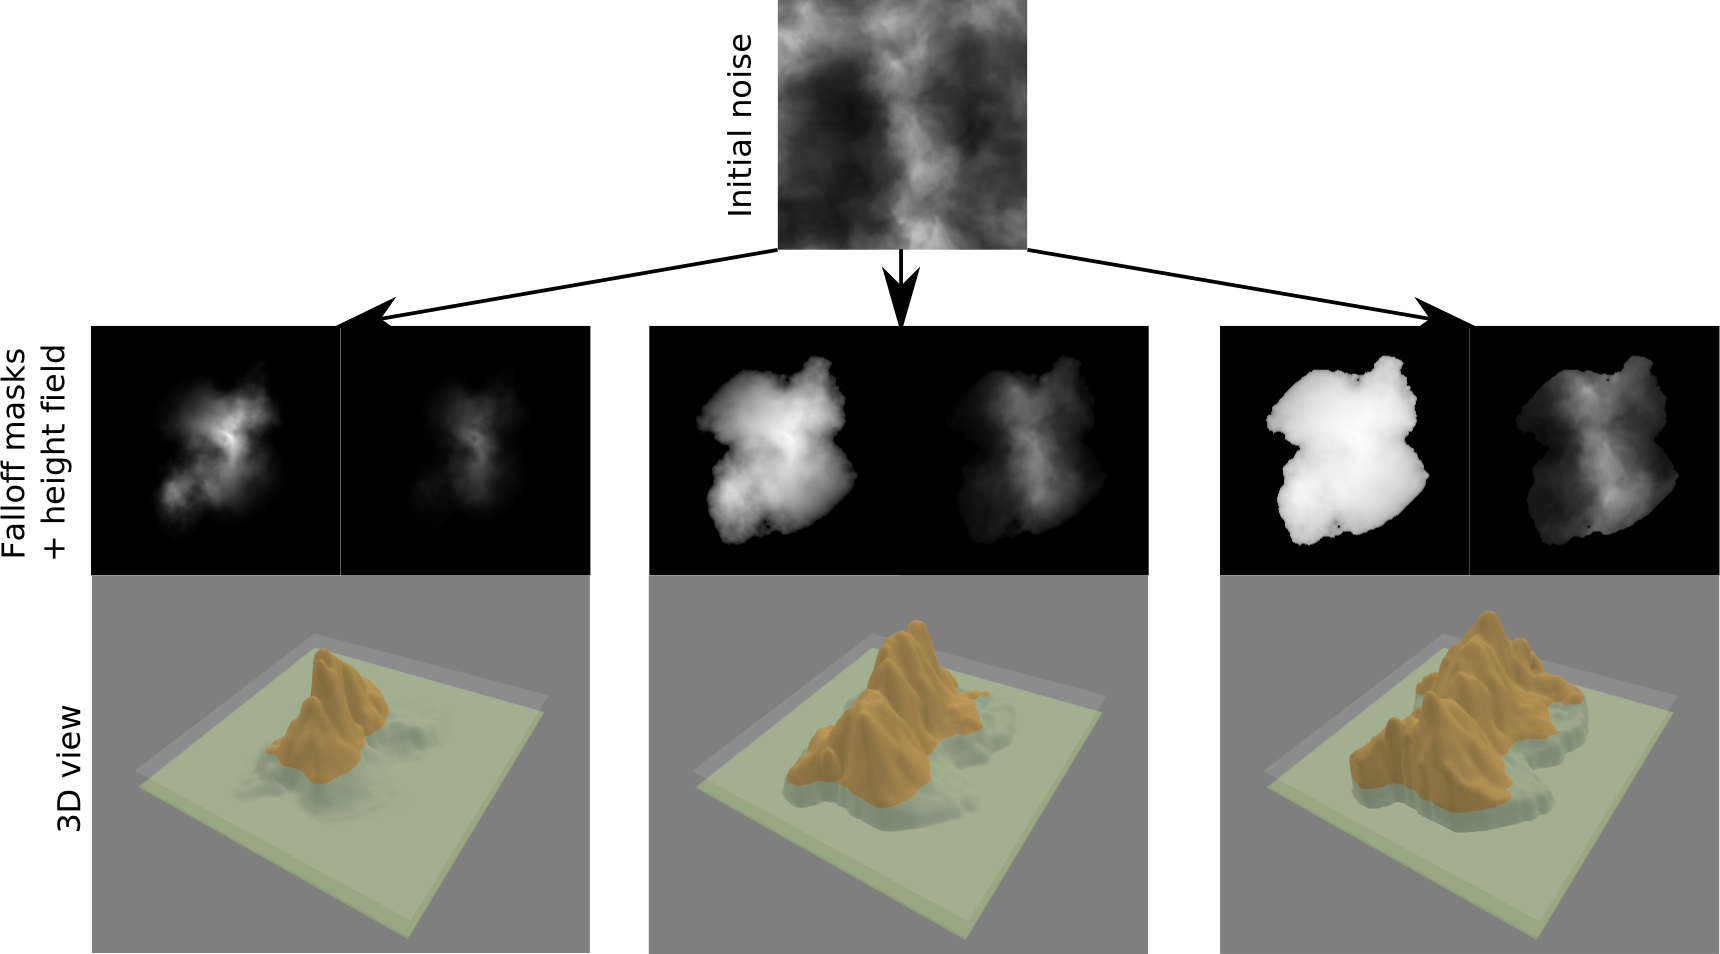
\includegraphics[width = \linewidth]{noise_examples3.pdf}
\caption{Three different results of an island generated from noise functions. In each case, the initial height field is the same, computed through flow noise. The falloff masks are also generated with a combination of fBm noise mitigated by the Euclidean distance from the image centre, warp noise and gamma correction. The only parameter modified for each example is the gamma correction. The results are very different, and hardly controllable. It is also difficult to represent lagoons and reefs using this method.}
\label{fig:coral-island-noise-example}
\end{figure}

Noise-based procedural generation remains one of the most widely used techniques for creating natural-looking terrains. Perlin noise \cite{Perlin1985}, Simplex noise \cite{Perlin2001}, and the Diamond-square algorithm \cite{Fournier1982} are foundational algorithms that generate pseudo-random yet continuous variations across a grid, producing terrain features that resemble organic landscapes. These techniques have been widely adopted in computer graphics and game development due to their efficiency and visual appeal.

Beyond basic noise functions, more advanced techniques such as fractal Brownian motion (fBm) and multifractal noise have been introduced to add finer-scale variation and detail \cite{Musgrave1989,Ebert2003}. fBm combines multiple layers, or "octaves," of noise at different frequencies and amplitudes, producing terrains that exhibit more realistic and varied features. The combination of noise with domain warping and signal processing techniques has been explored in depth in procedural modelling literature \cite{Reinhard2010}, enabling further control over visual complexity and terrain realism.

Noise functions are often paired with falloff maps to produce island-like terrains, where elevation gradually decreases towards the edges of the domain, mimicking coastlines and basic island shapes (see \cref{fig:coral-island-noise-example}). Various methods for enhancing island generation using noise and falloff blending have been proposed for applications in games and virtual worlds \cite{Olsen2004}. While these techniques excel at producing large, visually diverse landscapes quickly, they suffer from several key limitations when applied to the modelling of coral reef islands.

Critically, noise-based terrains lack grounding in geological or biological reality. They generate spatial patterns through mathematical noise, not through simulations of real-world processes such as volcanic subsidence or coral accretion. The signal processing parameters typically involved (frequency, lacunarity, gain, amplitude, ...) are tuned for visual effect rather than scientific plausibility. As highlighted in procedural modelling surveys \cite{Smelik2009,Galin2019}, this disconnect results in a lack of semantic control and poor correlation with actual environmental dynamics, making it difficult to represent phenomena like reef rings, lagoons, or atoll structures in a biologically or geologically coherent way.

Moreover, the biological aspects of coral growth are inherently tied to environmental conditions. Coral reefs form and persist only within specific ranges of water depth, sunlight, salinity, and water quality. Their growth patterns are further influenced by ecological health, nutrient availability, and symbiotic relationships. These dependencies are extremely difficult to capture in procedural noise systems, which are not designed to model such complex and coupled dynamics.

Our approach goes beyond the randomness of noise-based generation by incorporating real-world geological and biological processes into the terrain formation pipeline. Specifically, we model the gradual subsidence of volcanic islands and the upward growth of coral reefs, both of which are central to the long-term evolution of coral reef islands. By embedding these natural processes directly into the generation algorithm, we produce terrains that are not only more realistic but also more controllable. This integration of scientific modelling with procedural flexibility allows us to overcome the inherent limitations of traditional noise-based techniques and more accurately represent the complex formation of coral reef island systems.

\subsubsection{Simulation-based modelling}

Simulation-based terrain modelling methods aim to increase realism by replicating natural processes such as erosion, sediment transport, tectonic uplift, and vegetation growth. Unlike noise-based techniques, which rely on random functions, simulation-based approaches model causality and temporal dynamics to describe how a terrain evolves over time under physical or biological forces. These methods are often used to enhance base terrains, adding geologically plausible detail and structure \cite{Benes2006, Smelik2009}.

\subsubsubsection{Hydraulic and thermal erosion}

Hydraulic erosion models simulate the impact of flowing water on the landscape by modelling erosion, sediment pickup, transport, and deposition. Early implementations by \cite{Musgrave1989} laid the groundwork for erosion in procedural generation, while more recent works have accelerated these simulations using GPU architectures \cite{Mei2007} and particle-based methods \cite{Neidhold2005}. These simulations often follow Eulerian fluid models or Lagrangian particle systems to capture terrain displacement.

Thermal erosion, by contrast, simulates mass movement due to gravity, redistributing material from steeper slopes to gentler gradients, akin to landslides or soil creep \cite{Benes2006}. These erosion models generate realistic fluvial networks and landforms, but they are parameter-sensitive and computationally expensive.

Moreover, such models are generally designed for terrestrial landscapes and lack mechanisms for simulating underwater sedimentation, reef growth, or biogenic processes crucial to coral island formation. These models typically simulate time scales relevant to geomorphological processes (hundreds to thousands of years), which are mismatched with both the faster dynamics of biological processes like coral health and the slower geological evolution of reef islands.

We will propose our new particle-based erosion simulation method, adapted for underwater and terrestrial landscapes, in \cref{chap:erosion}.

\subsubsubsection{Tectonic uplift and geologic simulation}

Geological simulation approaches such as those proposed by \cite{Cordonnier2016, Cordonnier2017a} and extended by \cite{Schott2023} model terrain evolution through crustal deformation and tectonic uplift. These methods simulate isostatic adjustments, plate tectonics, or local uplift phenomena, often over geological timescales.

Although well-suited for mountain-building processes or fault line modelling, these methods are not designed to account for biogenic terrain formation, such as coral reef accretion, which is critical for simulating coral reef islands. As a result, despite being physically grounded models, they do not capture the coupled geological and biological dynamics necessary for representing the long-term evolution of reef islands.

\subsubsubsection{Vegetation and ecosystem dynamics}

Some simulation-based terrain models integrate ecological dynamics to reflect the feedback between terrain and living systems. For instance, \cite{Ecormier-Nocca2021} and \cite{Cordonnier2017b} simulate interactions between vegetation and terrain erosion, modelling plant colonisation, growth, and their influence on soil stability and moisture retention.

These ecosystem simulations allow more complex landscape evolution by considering biotic agents; however, they are designed primarily for terrestrial plants and temperate ecosystems. Coral colonies, in contrast, are marine organisms with strict environmental requirements such as limited depth, adequate sunlight, warm water temperatures, and clear water for photosynthesis via symbiotic algae. Accurately simulating these dependencies would require significant computational resources.

Furthermore, coral growth is not a passive process like sediment accumulation or root expansion, but an active accretion system that builds calcium carbonate structures over thousands of years. These unique growth mechanisms, constrained by marine ecology, fall outside the scope of existing vegetation or soil–plant–water feedback models.

\midConclusion

While simulation-based models represent a significant advancement over purely procedural approaches, they fall short in capturing the coupled geological and biological dynamics that shape coral reef islands. They are either computationally intensive, domain-specific, or biologically inapplicable, highlighting the need for a new class of terrain generation tools that embed long-term marine biogeomorphological processes into the procedural pipeline.




% \comment{Here, present hydraulic erosion (which will be developed indepth in \cref{chap:erosion}), then uplift simulation \cite{Cordonnier2017a,Cordonnier2016} and \cite{Schott2023}, then \cite{Ecormier-Nocca2021} and \cite{Cordonnier2017b} for simulating erosion + vegetation, but coral does not behave like a vegetal, nor fauna, nor geology. }



\subsection{Sketch-based terrain modelling}
\label{sec:coral-island-sota-sketches}

The term sketching encompasses several meanings: it can refer to performing gestures with the hand or body, creating a rough drawing, or outlining an idea in a simplified form. Accordingly, sketch-based modelling in 3D computer graphics can be understood through three complementary perspectives, each centred around a distinct core concept.

First, sketching may focus on interaction, where gestures captured through hand or body motion are used to manipulate virtual objects, often in immersive environments like virtual or augmented reality, drawing on established techniques such as sculpting and distortion \cite{Olsen2009, Cook2009}. Second, it can involve construction, where simple geometric primitives (curves, parametric shapes, implicit surfaces, ...) are combined under constraints to build more complex models. Finally, sketching may centre on interpretation, where the user draws strokes on a 2D canvas and the system analyses their meaning to generate a plausible 3D model.

While sketch-based modelling encompasses a wide range of techniques, including gesture-driven interaction in immersive environments, this work focuses primarily on the construction and interpretation aspects. In particular, construction serves as the foundation for procedural generation techniques using geometric primitives and constraints (addressed in this section), while interpretation becomes relevant when exploring data-driven approaches using deep learning to infer terrain structure from sketches (discussed in the following section). Interaction-based techniques, though significant in other contexts, fall outside the scope of this work.

To distinguish clearly between the different aspects addressed in this chapter, we will refer to the constructive approach as sketch-based, and to the interpretive, learning-driven approach as learning-based. It is important to note, however, that the boundaries between these categories are inherently blurry and often overlap in practice.

In procedural terrain generation, sketch-based construction approaches enable users to shape landscapes by manipulating high-level geometric primitives through intuitive sketching interfaces. These methods allow the definition of key terrain features, such as mountains, valleys, and coastlines, by drawing their outlines on a two-dimensional canvas, which are then procedurally transformed into 2.5D or 3D terrain representations. This approach offers a high degree of artistic control, making it particularly effective for creative applications like video games and simulations, where modelling is primarily user-driven.

\subsubsection{Curve-based modelling}

Sketch-based terrain generation often begins with user-defined curves that act as high-level constraints to guide the shape of the terrain. These curves may represent silhouettes, ridgelines, valleys, or feature outlines. Once defined, they are interpreted by the system and translated into elevation changes through various computational techniques. This approach allows for intuitive control over large-scale landforms while maintaining a procedural foundation for terrain synthesis.

\AltTextImage{
One of the earliest and most influential works in this domain is the system introduced by \citep{Gain2009} (\cref{fig:coral-island-Gain2009}), which enables users to sketch silhouettes, ridges, and spine curves to define complex terrain structures. The method employs multiresolution surface deformation and propagates wavelet-based noise from the sketched features to their surroundings, allowing users to generate detailed, natural-looking terrains from minimal input. This approach demonstrated the effectiveness of combining intuitive sketch input with procedural detail synthesis.

We draw direct inspiration from this work's dual-view sketching strategy, combining top-view and profile sketches, which closely aligns with our concentric curve and height-profile input approach.

Expanding on this idea, \citep{Hnaidi2010} proposed a technique based on diffusion equations. In their method, curves are annotated with geometric constraints such as elevation or slope, and a diffusion process is used to interpolate these constraints across the terrain surface. This results in smooth, continuous elevation fields that conform to user-defined features such as rivers, ridgelines, or cliffs. The use of parameterised curves as terrain anchors allows for precise control over landform shaping, while maintaining a high degree of automation.

}{sketchingGain2009-vertical.png}{\cite{Gain2009} propose to edit terrains through sketching by diffusing a noisy height function over a bounded region, effectively modelling mountain ranges.}{fig:coral-island-Gain2009}

\AltTextImage{
In a different interaction paradigm, \citep{Tasse2014} introduced a first-person sketching interface, where users draw terrain silhouettes from a particular camera viewpoint (\cref{fig:coral-island-Tasse2014}). These silhouettes are then projected into 3D, and a deformation algorithm adjusts the terrain so that the drawn features are visible exactly as intended from the user's perspective. This method supports complex silhouettes with occlusions, T-junctions, and cusps, and represents a more immersive and perceptually grounded approach to sketch-based terrain editing.
}{sketchingTasse2014-vertical.png}{\cite{Tasse2014} use sketching in association with camera position and direction to constrain the edition of height fields.}{fig:coral-island-Tasse2014}

These methods demonstrate the expressive power of curves as terrain-defining elements. By enabling users to sketch intuitive shapes and constraints, they bridge the gap between artistic intent and procedural complexity. Curve-driven approaches remain foundational in terrain modelling, particularly when user control over large-scale structure is essential. While we do not use the diffusion model, the idea of sketch-defined elevation constraints along curves informs our use of user-defined shape boundaries.

\subsubsection{Constraint-based modelling}

While curve-driven techniques provide intuitive shape design, constraint-based and gradient-based approaches focus on exerting precise control over terrain features through formal specifications such as elevation values, slopes, or gradient fields. These methods prioritise structural accuracy and procedural consistency, making them particularly suited to applications that demand terrain realism, integration with geographic data, or fine-grained editing capabilities.

\AltTextImage{
A representative example of constraint-based modelling is presented by \citep{Gasch2020}, who propose a method for procedural terrain generation that respects user-defined elevation constraints (\cref{fig:coral-island-Gasch2020}). Their system allows users to fix values at specific control points (e.g., paths, landmarks) and then employs a system of equations to propagate these constraints throughout the terrain. Crucially, the method integrates these constraints with a noise-based procedural function to preserve natural randomness while conforming to user intent. This approach is especially valuable when generating terrains that must align with real-world data or gameplay constraints.

We do not adopt their constraint-solving mechanism, but conceptually relate our profile sketch input to a localised height constraint.

}{sketching-Gasch2020.png}{\cite{Gasch2020} use a top-view sketch to apply constraints (a) on the noise function modelling a terrain, creating an intuitive means to create paths and roads in the resulting terrain (b and c).}{fig:coral-island-Gasch2020}

\AltTextImage{
Extending the idea of constrained procedural generation, \citep{Talgorn2018} introduce a real-time sketch-based terrain generation system based on a GPU-accelerated implementation of midpoint displacement. Users sketch curves with explicit elevation values, which act as absolute constraints, while the system extrapolates and interpolates terrain surfaces in real-time. Moreover, the user input can influence the elevation constraint and interpolation method properties of the midpoint displacement algorithm using the Red, Green and Blue channels (\cref{fig:coral-island-Talgorn2018}). Crucially, their model supports both global and local control over interpolation curvature and roughness, and introduces semantic labelling of sketched features (e.g., ridges vs. rivers) to influence how terrain propagates around constraints. This combination of sketch-based input, constraint propagation, and semantic control enables expressive, large-scale terrain modelling at interactive speeds. We do not reuse their fractal interpolation model, but we incorporate their notion of semantic labels and hierarchical constraint propagation to support real-time terrain shaping with sketch-defined features.
}{sketching-Talgorn2018.png}{\cite{Talgorn2018} use top-view sketching to encode properties in the noise function used to model the terrain surface.}{fig:coral-island-Talgorn2018}

\AltTextImage{
Building on the need for more intuitive editing, \citep{Guerin2022} introduce a novel paradigm by modelling terrain in the gradient domain. Rather than specifying elevation values directly, users interact with slope-based representations, allowing for the manipulation of terrain inclination and the integration of local edits into global terrain structure (\cref{fig:coral-island-Guerin2022}). By controlling terrain gradients and reconstructing elevation through integration, this method enables seamless blending between regions and supports a more natural editing workflow, particularly for sculpting realistic mountain ridges, valleys, or plateaus.
This gradient-domain editing approach offers interesting insights, but is not directly used, as we operate in the elevation domain with semantic control.
}{sketching-Guerin2022-vertical.png}{\cite{Guerin2022} apply gradient and height constraints on curves and diffuse them on the terrain to create landscapes with lightweight and multi-scale representations.}{fig:coral-island-Guerin2022}

Both approaches offer complementary strengths: constraint-based methods ensure precise adherence to user-defined features or data sources, while gradient-based systems provide fluid, perceptual control over terrain shaping. Together, they represent a shift toward high-level modelling tools that maintain procedural expressiveness while granting users a deeper degree of terrain control.

\subsubsection{Semantic terrain representation}

Beyond geometric sketching and low-level constraints, a third class of methods explores high-level terrain construction, where users guide terrain generation using abstract or semantic inputs. These approaches aim to simplify the authoring process by allowing users to describe what a terrain should contain (e.g., a mountain or a valley) without specifying how to generate it geometrically. Such methods often rely on symbolic sketching, sparse representations, or domain-specific visual cues, offering powerful tools for conceptual design and inverse procedural modelling.

\AltTextImage{
In this vein, \citep{Genevaux2015} propose a method for representing terrains as sparse combinations of procedural primitives, referred to as "terrain atoms." These atoms are stored in a dictionary and can be either extracted from real-world data or generated synthetically. The terrain is modelled as a linear combination of these features, forming a Sparse Construction Tree that blends primitives in a compact and expressive form (\cref{fig:coral-island-Genevaux2015}). This representation facilitates terrain editing, amplification, and reconstruction from coarse user input.
While this work introduces a symbolic representation of terrain via atoms, it is not reused in our method, which instead relies on semantic label maps.
}{sketching-Genevaux2015-1.png,sketching-Genevaux2015-2.png}{\cite{Genevaux2015} symbolically define a terrain by an aggregation of patches with real-world meaning.}{fig:coral-island-Genevaux2015}

\AltTextImage{
A more illustrative and domain-specific use case is presented by \citep{Natali2012}, who introduce a system for rapid visualisation of geological concepts. Here, users sketch schematic representations of subsurface structures such as faults, folds, or strata, and the system generates plausible 3D visualisations of geological terrains (\cref{fig:coral-island-Natali2012}). The tool is designed primarily for educational and exploratory purposes, enabling geoscientists and students to create, manipulate, and communicate complex geological scenarios through intuitive sketch input. Although it extends beyond traditional terrain elevation modelling, the work exemplifies how sketch-based systems can operate on a conceptual level and support domain-specific semantics.
This work inspired our use of sketch strokes to define deformation fields, although our implementation targets structured terrain generation rather than schematic visualisation.
}{sketching-Natali-2012.png}{\cite{Natali2012} use sketching to describe geological phenomena such as (top) geological layer deformation, (middle) abrupt displacement from faulting, and (bottom) texture deformation.}{fig:coral-island-Natali2012}

These high-level approaches demonstrate the potential of sketch-based modelling not just as a geometric tool, but as a semantic interface between human intention and terrain synthesis. By abstracting terrain construction into symbolic or feature-based representations, they allow users to create rich, expressive landscapes without directly engaging with low-level geometry, making them particularly valuable for tasks involving conceptual design, education, and inverse procedural modelling.

\midConclusion

The works presented in this section illustrate the diversity of sketch-based approaches for constructive terrain modelling, from curve-driven shape control to constraint-based editing and semantic abstractions. While these methods offer valuable tools for intuitive user interaction and procedural shaping, they often lack ecological grounding, multi-view integration, or the ability to produce structured data suitable for training generative models. In our work, we reinterpret and adapt elements from these approaches such as dual-view sketching, curve-based region definition, and deformation fields, to support the generation of coral reef islands through a hybrid procedural and learning-based pipeline. This constructive sketch-based foundation enables us to balance user control with scalable terrain generation in data-sparse domains.

% \comment{Also need to include \citep{Ketabchi2016}}


\subsection{Deep learning}
\label{sec:coral-island-sota-deep-learning}

\begin{figure}[H]
\centering
\includegraphics{schemaGAN_cGAN.jpg}
\caption{The general structure of GAN and cGAN networks is similar: a generator network $G$ is trained to take some noise $z$ as input to try to create a "realistic" output $X_{\text{fake}}$, and a discriminator network $D$ is trained in parallel to distinguish generated data from real data. cGAN networks introduce a class input $c$, used by both the generator and discriminator in their inference process. In the end, only the generator is used to create new data.}
\label{fig:coral-island-GAN-scheme}
\end{figure}

Over the past decade, deep learning has revolutionised many areas of computer graphics and procedural content creation by learning complex, data-driven priors directly from examples. Unlike purely procedural or sketch-based methods, which rely on hand-tuned noise functions or geometric constraints, neural networks can capture subtle patterns and high-frequency details without explicit programming of each effect. In terrain synthesis, this enables models to infer realistic elevation structures, textures, and region transitions from training data, even when that data is sparse or synthetic. In the context of coral reef islands, where high-resolution digital elevation models are rare, deep learning offers a way to abstract away low-level procedural rules and directly learn the mapping from semantic layouts (label maps) to plausible height fields. In the following sections, we first review general Generative Adversarial Networks (GANs) and then focus on their conditional variant (cGAN), which forms the backbone of our sketch-to-terrain translation pipeline.

\subsubsection{Generative Adversarial Networks}
\label{sec:coral-island-sota-GAN}

Generative Adversarial Networks (GANs), introduced by \cite{Goodfellow2014}, are a class of generative models in which two neural networks are trained in opposition: a generator $G$ learns to produce synthetic data samples that resemble those from a target distribution, while a discriminator $D$ learns to distinguish real samples from those generated. Through this adversarial process, the generator improves its ability to mimic the underlying data distribution, enabling the creation of realistic outputs from random input.

GANs have been widely adopted for image synthesis, texture generation, and data augmentation, among other tasks. In terrain modelling, they offer the potential to generate plausible landforms by learning directly from real-world data, without requiring hand-crafted procedural rules. The following works demonstrate how different GAN variants have been applied to terrain synthesis, each with its own assumptions, design trade-offs, and limitations.

Early applications of GANs to terrain focused on unconditional generation, where elevation maps are synthesised from pure latent noise, without any spatial or semantic guidance. \citep{WulffJensen2018} trained a deep convolutional GAN (DCGAN) to produce realistic digital elevation models of mountainous landscapes, showing that terrain-like structures could emerge from purely data-driven learning. The model captured local elevation statistics and allowed for latent space interpolation, enabling smooth variations across generated terrains. However, the lack of spatial conditioning made it difficult to control or constrain specific features such as ridges, valleys, and coastlines, resulting in landscapes that reflected training set distributions but offered no means for intentional design.

\citep{Spick2019} extended this approach by introducing a Spatial GAN that generates height and texture maps jointly. By conditioning the generation process on spatial coordinates, their model enforced local consistency and reduced structural artefacts. This integration simplified the content pipeline by fusing geometry and appearance into a single pass. Yet despite improved quality, the generation process remained fundamentally uncontrolled: there was no way for users to specify terrain layout, features, or semantics. As with earlier GANs, the model learned to mimic terrain distributions but could not support authoring or guided synthesis.

To address the lack of control inherent in purely noise-driven GANs, later works introduced multi-stage architectures in which a second, conditional GAN refines or interprets the output of a first-stage generator. \citep{Beckham2017} proposed a two-step pipeline where a DCGAN generates bare terrain heightmaps from noise, and a conditional pix2pix network adds texture based on semantic cues. This separation of geometry and appearance allows for basic stylisation and terrain remixing, but still suffers from the lack of control in the initial heightmap generation. In a conceptually similar structure, \citep{Panagiotou2020} reversed the mapping: an unconditional GAN first synthesises aerial RGB imagery from noise, which is then passed to a cGAN trained to predict plausible DEMs. While this image-to-DEM translation enables realistic terrain reconstruction, it depends on large collections of paired data and lacks any semantic or structural control from the user. In both cases, despite the introduction of a conditional refinement stage, the generation process remains fundamentally anchored in an unconstrained latent input, offering limited authoring capability and no principled way to shape landform structures.

These approaches show a shift towards using conditional models to guide terrain generation with more structure. But because they still start from random noise, they offer little real control over the layout or meaning of the terrain. A natural next step is to guide the generation process directly from user-defined semantic inputs, such as sketches or label maps, to produce terrain that reflects both the training data and the user's intent.


\subsubsection{Conditional GANs for terrain generation}
\label{sec:coral-island-sota-cGAN}

While traditional GANs generate data from noise, Conditional GANs (cGANs) extend this concept by incorporating side information, often called a class map or label map, to guide generation toward user-specified outcomes \cite{Mirza2014}. This makes them particularly attractive for structured content synthesis tasks, including terrain generation, where user input often defines large-scale layout while realism must emerge from learned detail. The pix2pix framework by \citep{Isola2017} is the canonical cGAN formulation for image-to-image translation. It uses a U-Net generator conditioned on an input image (a sketch or a label map, for example), and a PatchGAN discriminator that evaluates realism at the patch level, encouraging fine detail and local consistency (\cref{fig:coral-island-pix2pix-example} presents two image-to-image translations from the same pix2pix network architecture).

\begin{figure}[H]
\centering
\includegraphics[width = 0.8 \linewidth]{example_pix2pix_facade.png}
\includegraphics[width = 0.8 \linewidth]{example_pix2pix_maps.png}
\caption{Example of pix2pix image-to-image translation: (top) a trained model converts semantic label maps into realistic façade images, and (bottom) constructs highly plausible aerial images from navigation map sketches. This paradigm generalises to many tasks, including terrain generation.}
\label{fig:coral-island-pix2pix-example}
\end{figure}

In the domain of terrain generation, the use of cGANs remains surprisingly rare. The most directly relevant precedent is the work of \citep{Guerin2017}, who train a pix2pix-style cGAN to map sketched terrain features such as valleys, ridgelines, or peaks into full-resolution digital elevation models (DEMs). Their results demonstrate that cGANs can plausibly reconstruct complex topographic forms from sparse semantic cues, offering a promising balance between user control and learned realism. Similarly, \citep{Sisodia2022} apply a cGAN to generate stylised terrain heightmaps from sketch maps in the context of 2D game environments, further validating the sketch-to-terrain pipeline.

Another related line of work explores learning-based terrain synthesis using partial or sparse spatial inputs. \citep{Voulgaris2021} propose a GAN-based system that maps sparse "altitude dot" maps to plausible terrain imagery, acting as a minimal-interaction generative authoring tool. While not strictly a cGAN, their system reflects a similar spirit: conditioning generation on lightweight user constraints. Likewise, \cite{Panagiotou2020} and \cite{Beckham2017} train a cGAN to invert RGB satellite imagery into elevation data, framing terrain modelling as an appearance-to-geometry and geometry-to-appearance translation task. However, such image-to-DEM (and DEM-to-image) systems are heavily dependent on large paired datasets, which limits their applicability in settings like coral reef islands, where training data are scarce.

Despite this emerging body of work, there is still no standard pipeline for generating detailed terrains from semantic layout maps using cGANs, particularly in biologically driven environments like coral reef islands. This gap is outstanding given the success of cGANs in analogous image synthesis domains, and the explosive progress in the field of deep generative models. The potential of this approach remains underexploited, especially when it comes to coupling user control with long-term geological plausibility.

\midConclusion

In our method, we address this gap by training a pix2pix cGAN to transform label maps (semantic region maps produced by procedural sketch-based modelling) into realistic coral reef island height fields. Each input map encodes key zones of an island (e.g., lagoon, reef crest, beach, island core) using categorical labels, serving as semantic constraints for terrain synthesis. The cGAN generator learns to condition elevation details on both the global layout and the implicit patterns encoded in the training data. By generating our own synthetic dataset with procedurally modelled coral islands (see \cref{fig:coral-island-difficulties-dataset}), we overcome the shortage of labelled elevation data and enforce geological coherence via data generation design.

This setup offers several key advantages: it respects user-defined structure while allowing the generator to introduce realistic variation; it removes procedural biases such as radial symmetry and fixed island typologies; and it enables the generation of irregular, non-circular landforms while implicitly modelling geological processes like subsidence and coral accretion through training-time priors.

In this context, conditional GANs emerge as a powerful yet underutilised tool for terrain modelling. By training on procedurally generated coral island data, we show that sketch-conditioned learning can effectively bridge the gap between high-level user intent and geologically plausible terrain synthesis.




\section{Description of our method}
\label{sec:coral-island-method-description}

\begin{figure}[H]
\includegraphics[]{pipeline_full.pdf}
\caption{Our pipeline first prompts the user to create single pairs of coral reef island height fields and label maps using our proposed curve-based modelling algorithm (\cref{sec:coral-island-example-generation}). The same algorithm is applied multiple times on randomly altered versions of the user input to create a dataset, which we further enhance with data augmentation techniques (\cref{sec:coral-island-dataset-generation}). Finally, we train a conditional Generative Adversarial Network, which can then be used standalone to create height fields from labelled sketches (\cref{sec:coral-island-cGAN-training}).}
\label{fig:coral-island-pipeline}
\end{figure}

% Our method for generating coral reef islands combines user-driven sketching, procedural techniques, and deep learning to create realistic and varied island terrains (\cref{fig:coral-island-pipeline}). 

% The pipeline consists of two distinct phases: a procedural data-generation phase and a deep-learning-driven inference phase. 

% \subsection{Procedural generation phase}
% \label{sec:coral-island-proc-phase}

% In the initial procedural phase, the user sketches key island features from two complementary viewpoints: a top view, defining the horizontal layout of island features (island boundaries, beach width, lagoon areas, coral reefs), and a profile view, specifying the vertical elevation profile from island center to ocean (\cref{sec:coral-island-generation-initial}).

% Additionally, users can sketch a wind deformation map, enabling simulation of natural erosion patterns caused by wind and waves (\cref{sec:coral-island-wind-deformation}).

% From these sketches, the procedural system generates a synthetic island terrain with the keep-up stategy of coral reefs (\cref{sec:coral-island-coral-reef}) and a corresponding semantic label map, where each pixel indicates its region type (island, beach, lagoon, reef, abyss) (\cref{sec:coral-island-procedural-output}).




% \subsubsection*{User interaction}
% \label{sec:coral-island-description-UI}

% \begin{figure}[H]
%     \centering
%     \includegraphics[width = 0.9 \linewidth]{user_interaction_generation.png}
%     \caption{The user can interact directly on the island by editing the different canvases in no specific order. This UI shows, from left to right, the top-view sketch with the different outlines of each regions, the profile-view sketch with the outlines represented in dotted lines, the wind velocity sketch drawn with strokes (last stroke is visible), and the resistance function showing here a high resistance at the top of the island and on the front reef.}
%     \label{fig:coral-island-wind-from-strokes-interaction}
% \end{figure}

% As users draw the top-view and profile-view sketches, the system provides real-time feedback on the resulting terrain. The top-view sketch influences the horizontal layout of the island, while the profile-view sketch defines its vertical structure. These sketches can be adjusted independently, allowing the user to fine-tune both the outline and elevation of the island.

% While sketching the basic shape, users can apply wind deformation strokes to modify the island's features further. These strokes represent wind and wave influences, distorting the island's shape to introduce more natural, non-radial features such as indentations along the coastline, variable lagoon shapes, or concave formations. The system automatically applies these deformations, providing real-time feedback as the user interacts with the terrain.

% This interactive process, combining sketches and wind deformation, allows users to quickly iterate on their designs, refining the terrain to meet specific aesthetic or functional goals.


% \comment{Add output description from full procedural}

% \subsection{Learning-based generation phase}
% \label{sec:coral-island-cGAN-phase}

% We repeat this procedural generation process many times with varied parameters (different shapes, scales, subsidence levels, and wind patterns) to create a large synthetic dataset (\cref{sec:coral-island-dataset-generation}). Each dataset entry consists of a label map paired with its procedurally generated terrain height field. Data augmentation is applied to the generated pairs to reduce the impact of the constraints induced from the procedural method (\cref{sec:coral-island-data-augmentation}).

% We use this dataset to train a Conditional Generative Adversarial Network (cGAN), specifically the pix2pix architecture, capable of translating label semantic maps into realistic terrain height fields (\cref{sec:coral-island-cGAN-output}).

% After training, the procedural step becomes unnecessary. To generate new island terrains, the user only needs to provide a label semantic map as input to the trained cGAN. The cGAN then synthesizes realistic island elevation details directly, capturing learned geological and geomorphological patterns from the synthetic training data (\cref{sec:coral-island-results}).

% \subsubsection*{User interaction}
% \label{sec:coral-island-cGAN-phase-interaction}

% Thus, the trained cGAN provides a user-friendly interface: users draw or edit simple label maps (regions) to rapidly generate diverse, geologically plausible coral reef island terrains, incorporating realistic features such as smooth transitions between regions, detailed coral reef structures, and naturally varied shapes free from procedural constraints.

% \midConclusion

% This combined procedural-and-learning approach provides a simple, flexible, and powerful tool for island terrain generation, enabling users to intuitively generate realistic and diverse coral reef islands aligned with real-world geological and biological processes such as volcanic subsidence, coral reef growth, and wind-driven erosion.


Our method for procedural generation of coral reef islands is composed of two independent modelling techniques shown in \cref{fig:coral-island-pipeline}. A first curve-based algorithm (top-left blue block, presented in \cref{sec:coral-island-example-generation}) parametrises the surface of islands via a top-view sketch interface, describing the outlines of its constituent regions and a stroke-based wind field deforming them, as well as a profile-view sketch describing, for each region, its altitude and resistance to deformations. User inputs are given as 1D functions (altitude and resistance), a 1D polar function (island outlines), and a 2D vector field (wind field), as shown in \cref{fig:coral-island-wind-from-strokes-interaction}, which are convenient to randomise through the use of noise, but limit the user's freedom to model arbitrary shapes.

We propose a second learning-based generation algorithm (right red blocks \cref{fig:coral-island-pipeline}, developed in \cref{sec:coral-island-cGAN-training}), which trains a neural generator $G$ to transform a labelled image into a height field. In parallel, a discriminator $D$ is trained to distinguish height fields provided from the training set against height fields generated by $G$. This adversarial training strengthens the outputs of the generator, up to the point where we discard the discriminator and training data, only keeping the generation step (bottom-right). Users are then able to provide unseen label maps and obtain height fields as close as possible to the training dataset. This method for terrain modelling is poorly constrained, however, and requires a large amount of prior data in its training set, which is not available in our case.

We connect these two algorithms through a process of dataset generation (central orange block \cref{fig:coral-island-pipeline}, described in \cref{sec:coral-island-dataset-generation}) in order to enforce the benefits of each while reducing their limitations. Given the initial curve-based user inputs, we create a dataset composed of similar samples processed by our first algorithm, rasterised into a 2D image of the parametrised regions, and paired with the resulting height field. We then greatly increase the size of the dataset by employing various data augmentation techniques such as translations, scaling, and copy-pasting of multiple islands in a single sample. We then obtain a dataset large enough for training our cGAN and enable users to procedurally create coral reef islands with a high level of control.

\begin{figure}
\centering
\includegraphics[width = 0.9 \linewidth]{user_interaction_generation.png}
\caption{The user can interact directly on the island by editing the different canvases in any order. This UI shows, from left to right: the top-view sketch with the different outlines of each region, the profile-view sketch with the outlines represented by dotted lines, the wind velocity sketch drawn with strokes (last stroke is visible), and the resistance function showing here a high resistance at the top of the island and on the front reef.}
\label{fig:coral-island-wind-from-strokes-interaction}
\end{figure}


























\section{Procedural island generation}
\label{sec:coral-island-example-generation}

The generation of coral reef island terrains involves a structured process that takes the user's sketches and produces a complete 3D terrain model. This process begins with the creation of the initial height field based on the user's input, followed by the application of wind deformation to introduce natural variations, and concludes with the integration of coral reef features through subsidence and coral growth modelling.

% \subsection{User inputs}
% \label{sec:coral-island-example-inputs}

The generation of coral reef islands in this system begins with two intuitive sketch-based inputs from the user: a top-view sketch and a profile-view sketch, which define the island's horizontal layout and vertical elevation profile. In addition to these sketches, the user can further refine the terrain by applying wind deformation strokes, which simulate the effects of wind and waves on the island's shape. This combination of sketches and wind inputs gives users precise control over both the island's structure and its natural variations, such as irregular coastlines or concave features. We will present the usefulness of these sketches in this section, and describe the technical details in the next section.

% \subsubsection{Top-view sketch}
% \label{sec:coral-island-top-view}
\subsection{Initial height field generation}
\label{sec:coral-island-generation-initial}

\begin{figure}[H]
\centering
\autofitgraphics[width=0.90 \linewidth]{Cicia_island.png, Cicia_island-outlines.png}
\autofitgraphics[width=0.90 \linewidth]{Cicia_island-3D.png}
\caption{(Left) A real-world example of aerial image (and 3D visualisation on bottom) of an island (Cicia Island) may be segmented into regions. (Right) We can represent the different regions by the boundaries they form.}
\label{fig:coral-island-top-view-sketch}
\end{figure}

The top-view sketch defines the island's outline as seen from above. Using a simple drawing interface, the user can delineate the boundaries between key regions of the island, including the island itself, the beaches, the lagoon, and the surrounding abyss. The system assumes that these regions are arranged concentrically around the centre of the island, with each boundary defined by a radial distance from the centre.

Each region's boundary is represented in polar coordinates, with $\radius_\p$ indicating the radial distance from the island's centre and $\angl_\p$ representing the angular position. This polar representation allows the system to map the user's sketch onto a circular framework, ensuring smooth transitions between regions and maintaining a coherent layout for the island.

In this sketch, the user defines the overall horizontal layout of the island, including the size and shape of each feature. Variations in the outline are introduced by allowing the radial distances to vary with angle, ensuring that the island is not strictly symmetrical and introducing more natural, irregular shapes.

\begin{figure}[H]
\autofitgraphics[]{binary-heights-input-only-outlines-2.png, binary-heights-output-only-heightmap-2.png, binary-heights-render-2.png}
\autofitcaptions{Input, Output, Rendered}
\caption{Using only the outlines of the island as an input sketch, we can provide a height to each point of the field depending on the region in which it lies.}
\label{fig:coral-island-procedural-height-only}
\end{figure}

% \subsubsection{Profile-view sketch}
% \label{sec:coral-island-profile-view}

\begin{figure}[H]
\centering
\autofitgraphics[]{profileFunction.pdf, schema_profile.jpg}
\caption{(Left) A profile function $\heightProfile$ is defined as a 1D function and represents the surface from the centre of the island to the abysses. (Right) The cross-section representation of an island is often represented as a 1D function defined using terrain features as landmarks.}
\label{fig:coral-island-profile-function}
\end{figure}

The profile-view sketch defines the vertical elevation profile of the island along any radial direction, offering control over the island's height. In this view, the user specifies the elevation of different regions of the island, such as the island peak, beach, lagoon, abyss, and everything in between, by drawing the corresponding profile curve.

The regions' outlines correspond to key terrain transitions: the highest point of the island (centre), the island border, the beach, the lagoon, and the deep-sea abyss. The system uses these milestones to interpolate a continuous 1D height function $\heightProfile(\distRegions)$, where $\distRegions$ represents a non-uniform region distance from the island's centre, and $h = \heightProfile(\distRegions)$ gives the height at each point. This continuous profile ensures smooth elevation transitions across the island.

By combining the top-view and profile-view sketches, the system can generate a full 3D terrain model that accurately reflects the user's design by revolution modelling.

The generation of the coral reef island terrain begins by transforming the user-defined top-view and profile-view sketches into a coherent 3D height field. This process combines the radial layout of the top-view sketch with the elevation information provided by the profile-view sketch, creating a terrain that accurately represents the desired features, such as the island, beaches, lagoons, and abyss.

For any point $\p$ on the terrain, the system computes polar coordinates $(\radius_\p, \angl_\p)$. The radial distance $\radius_\p$ determines which region the point belongs to (island, beach, lagoon, reef, or abyss) based on the user-defined radial limits. Those outlines from the top-view sketch provide the exact boundaries between regions.

Each point's height is computed using the profile function $\heightProfile(\distRegions)$. Instead of using the raw radial distance $\radius_\p$, we define a parametric region distance $\distRegions_\p$ that maps each point to a normalised position along the concentric regions (see \cref{fig:coral-island-parametric-distance}). The radial space is divided by user-defined boundaries $\Radius_0, \Radius_1, \dots, \Radius_n$, corresponding to the island centre, border, beach, lagoon, reef, and abyss.

\AltTextImage{
When a point $\p$ lies between two boundaries, say $\Radius_{i}$ and $\Radius_{i+1}$, its parametric distance is
\begin{align}
\distRegions_\p = i ;+; \frac{\radius_\p - \Radius_{i}}{\Radius_{i + 1} - \Radius_{i}},
\end{align}
where $i$ is the index of the region containing $\p$ (i.e., $\Radius_i \le \radius_\p < \Radius_{i+1}$). This linear mapping stretches each region's radial span to the interval $[i,,i+1]$, ensuring smooth interpolation across region boundaries. The final height at point $\p$ is then $h(\p) = \heightProfile(\distRegions_\p)$.
For any point $\p$, the height is finally computed as:
\begin{align}
h(\p) = \heightProfile(\distRegions_\p)
\end{align}
}{outlines-top-view-x-bar.pdf, outlines-result-x-bar.pdf}{The $\tilde{x}$ parameter is used to stretch the 1D height function $\heightProfile(x)$ to fit the distances from the centre to the outlines of each region defined in the top-view sketch.}{fig:coral-island-parametric-distance}



This approach ensures that the height field accurately follows the elevation profile specified by the user while maintaining smooth transitions between different regions of the island.

% \begin{figure}[H]
% \autofitgraphics[]{outlines-top-view-x-bar.pdf, outlines-result-x-bar.pdf}
% \caption{The $\tilde{x}$ parameter is used to stretch the 1D height function $\heightProfile(x)$ to fit the distances from the centre to the outlines of each region defined in the top-view sketch. }
% \label{fig:coral-island-parametric-distance}
% \end{figure}

The result is a height field that captures both the radial structure of the island (from the top-view sketch) and the vertical elevation profile (from the profile-view sketch), producing a realistic representation of islands with smooth transitions between the key terrain features.

\begin{figure}[H]
\autofitgraphics[]{smooth-input-outline-heights-1.png, smooth-output-heights-1.png, smooth-render-1.png}
\autofitgraphics[]{smooth-input-outline-heights-2.png, smooth-output-heights-2.png, smooth-render-2.png}
\autofitgraphics[]{smooth-input-outline-heights-3.png, smooth-output-heights-3.png, smooth-render-3.png}
\autofitcaptions{Input, Output, Rendered}
\caption{Providing a smooth function between each region results in islands with plausible reliefs. We fixed the outlines while editing only the height function in order to produce, from top to bottom, a low island, a coral reef island, and finally an identical island without the reef.}
\label{fig:coral-island-procedural-smooth-heights}
\end{figure}

\subsubsection{Wind deformation}
\label{sec:coral-island-wind-deformation}
% \subsubsection{Wind velocity field}
% \label{sec:coral-island-wind-view}

\begin{figure}[H]
\centering
\includegraphics[width = 0.8 \linewidth]{windByStrokes.pdf}
\caption{From the parametric curve defined by a user (red), we define the velocity field by considering the velocity (first derivative) of the curve at the closest point $\closestCp$, modulated by a Gaussian distance function $G_{\std}(x)$.}
\label{fig:coral-island-wind-from-strokes}
\end{figure}

In addition to the sketches, the user can influence the shape of the island by defining a wind velocity field. This field simulates the effects of wind and wave erosion on the island's surface, introducing natural deformations such as coastline indentations, and more importantly allows the user to break the radial symmetry constraint.

The wind field is represented as a series of wind strokes drawn by the user on a 2D canvas. Each stroke represents a parametric curve, where the direction and strength of the wind are encoded as a vector field. The user controls the wind's direction by drawing these curves, and the system interprets the strokes to create a velocity field that defines how the terrain should be deformed.

As the user draws a wind stroke, the system generates a set of control points along the curve, with the option to adjust the stroke's width. The width of each stroke determines the area of influence around the curve, where wider strokes result in broader deformations of the terrain.
The deformation strength decreases with distance from the wind curve using a Gaussian falloff function using the stroke width as standard deviation, ensuring that the terrain transitions smoothly from deformed regions to non-deformed areas.
Once the wind strokes are applied, the system processes the wind velocity field by displacing the terrain points accordingly. The height field, originally generated from the user's sketches, is modified by the wind field to create non-radial features, breaking the initial radial symmetry and producing a more organic island shape.








% \subsection{Generation process}
% \label{sec:coral-island-generation-process}
% The generation of coral reef island terrains involves a structured process that takes the user's sketches and produces a complete 3D terrain model. This process begins with the creation of the initial height field based on the user's input, followed by the application of wind deformation to introduce natural variations, and concludes with the integration of coral reef features through subsidence and coral growth modeling.

% \subsubsection{Initial height field generation}
% \label{sec:coral-island-generation-initial}
% The generation of the coral reef island terrain begins by transforming the user-defined top-view and profile-view sketches into a coherent 3D height field. This process combines the radial layout of the top-view sketch with the elevation information provided by the profile-view sketch, creating a terrain that accurately represents the desired features, such as the island, beaches, lagoons, and abyss.

% For any point $\p$ on the terrain, the system first computes the polar coordinates $(\radius_\p, \angl_\p)$, where $\radius_\p$ is the radial distance from the island's center, and $\angl_\p$ is the angular component. The radial distance $\radius_\p$ is used to determine which region the point belongs to (island, beach, lagoon, reef, or abyss). The user-defined outlines in the profile sketch specify the radial limits between these regions.

% Each point's height is determined by the profile function $\heightProfile(\distRegions)$, where $\distRegions$ represents a "piecewise parametric distance" from the island's center. The piecewise parametric distance works by dividing the radial distance from the center into segments, defined by these region boundaries. Each segment corresponds to a distinct region of the terrain, and within each segment, the distance $\distRegions$ is interpolated between the region boundaries. For a point $\p$ lying between two boundaries $\Radius_{i}$ and $\Radius_{i+1}$, the distance $\distRegions_\p$ is calculated as:

% \begin{align}
%     \distRegions_\p = i + \frac{\radius_\p - \Radius_{i}}{\Radius_{i + 1} - \Radius_{i}}
% \end{align}
% where $i$ is the index of the nearest lower region boundary. This method allows for smooth transitions between regions, even when the spacing between boundaries varies. 

% For any point $\p$, the height is finally computed as:
% \begin{align}
%     h(\p) = \heightProfile(\distRegions_\p)
% \end{align}

% This approach ensures that the height field accurately follows the elevation profile specified by the user while maintaining smooth transitions between different regions of the island.

% The result is a height field that captures both the radial structure of the island (from the top-view sketch) and the vertical elevation profile (from the profile-view sketch), producing a realistic representation of islands with smooth transitions between the key terrain features.



% \subsection{Wind deformation}
% \label{sec:coral-island-wind-deformation}

After generating the initial height field based on the top-view and profile-view sketches, the next step in the process introduces wind deformation. This step simulates the long-term effects of wind and wave erosion, breaking the radial symmetry of the terrain and adding natural variations such as concave coastlines and irregular island shapes.

The wind deformation can be controlled through a user-defined vector field, which represents the direction and strength of wind flows across the terrain. Users interact with the system by drawing strokes on a 2D canvas, which are then interpreted as parametric curves $\curve$ representing wind patterns. Each stroke defines a wind flow in the curve's direction $\curve'$, a strength $S$, and an effect width $\std$; these wind flows are used to displace the terrain, simulating the gradual reshaping of the island due to wind and wave erosion.

The strokes are represented as Catmull-Rom splines, a type of parametric curve that allows for smooth, continuous wind paths. For any point $\p$ on the terrain, the deformation vector $\warp(\p)$ is calculated based on the proximity of $\p$ to the nearest wind strokes. The strength of the displacement is controlled by a Gaussian scaling function, which ensures that points closer to the wind strokes experience stronger displacement, while points farther away are less affected.

The displacement function $\warp(\p)$ is computed as a sum of the influences from all nearby wind strokes. For each stroke, the deformation vector is scaled by a Gaussian function that smoothly decreases with the distance from $\closestCp$, the closest point on the parametric curve $\curve$, as follows:

\begin{align}
\warp(\p) = \sum_{\curve \in \text{curves}} S \frac{\curve'(\q)}{| \curve'(\q) | } \cdot G_\std\left(| \p - \closestCp | \right) % e^{-\frac{\norm{\p - \closestCp}^2}{2 \std^2}}
\
G_\std(x) = \frac{1}{\std \sqrt{2\pi}} e^{-\frac{x^2}{2 \std^2}}
\end{align}

Once the deformation vector $\warp(\p)$ is computed, the terrain height at point $\p$ is adjusted by displacing $\p$ to a new point $\warp(\p)$.
We can then compute the final height $h(\warp \circ \p) = \heightProfile(t_{\p})$, or, as the implicit modelling community would write it,
\begin{align}
\Tilde{h} = \warp^{-1} \circ h
\end{align}

This process introduces variations in the terrain, distorting the coastline, creating concave regions, and breaking the original radial symmetry defined by the top-view and profile-view sketches.

% \subsubsection{Resistance to deformation}
% \label{sec:coral-island-resistance}

\begin{figure}[H]
\centering
\includegraphics[width=0.45 \linewidth]{resistanceFunction.pdf}
\caption{The resistance function of the island is defined in the same way as the $\heightProfile$ function. The resistance to erosion and deformation arises from multiple factors such as depth, materials, wind shadowing, biotic and abiotic factors, ... Modelling all these factors is complex. As such, using a user-defined approximation through a resistance function $\resistance$ allows for more control.}
\label{fig:coral-island-resistance-function}
\end{figure}

To ensure that certain regions of the terrain, such as deep-water areas, remain relatively unaffected by the wind, a resistance function $\resistance(\distRegions)$ is applied. The resistance function modulates the effect of the wind deformation based on the previously computed piecewise parametric distance $\distRegions$, with the same interaction means as the $\heightProfile$ function.

The resistance function $\resistance(\distRegions)$ is defined similarly to the profile function, and it controls the magnitude of the displacement at each point. For example, regions near the coastline (such as the beach and lagoon) might have lower resistance, allowing for more significant deformation (simulating coastal erosion from wave energy), while regions farther away (such as the abyss) have higher resistance, limiting the wind and coastal erosion impact.

The deformation vector previously described is scaled by the resistance function at each point $\p$, such that the final deformation vector becomes:

\begin{align}
\Tilde{\warp}(\p) = \left(1 - \resistance(\distRegions_\p) \right) \cdot \warp(\p)
\end{align}

This ensures that the wind deformation has the greatest impact on areas like the coastline and beach, where erosion naturally plays a larger role, while deeper regions like the abyss or stronger regions like mountains remain stable and relatively unchanged.

\begin{figure}[H]
\autofitgraphics[]{result_low_resistance.png, result_high_resistance.png}
\caption{(Left) Given a uniform wind velocity field and a resistance function similar to \cref{fig:coral-island-resistance-function}, the coasts are smoothly eroded while the interior of the island is almost unaffected. (Right) Modifying the resistance function to affect a strong resistance to borders simulates the effect of coast reinforcements.}
\end{figure}

% \subsubsection{Deformation and height field update}
% \label{sec:coral-island-deformation}

The wind deformation process results in a modified height field where the terrain has been warped according to the user-defined wind strokes. This deformation introduces non-radial features, such as concave coastlines or irregularities along the beach and lagoon, making the island appear more natural and varied.

Both the height field and the label map (which tracks the terrain regions) are updated to reflect the wind deformation. This ensures that the semantic information of the terrain remains consistent even after the terrain has been warped. The label map is deformed in the same way as the height field, preserving the logical structure of the island for further post-processing, such as texturing.

For instance, consider a simple circular island generated from the initial height field. By applying wind strokes along one side of the island, the deformation process can create concave regions along the coastline, making the shape more irregular and mimicking the effects of real-world wind and wave erosion. The resistance function ensures that while the beach and lagoon areas are deformed, the abyss remains largely unaffected as they are far from the wind and wave effective areas, preserving the island's overall structure.

\begin{figure}
\autofitgraphics[]{wind-deform-input.png}
\autofitgraphics[]{wind-deform-output-original.png, wind-deform-render-original.png, wind-deform-output.png, wind-deform-render.png}
\caption{A top-view wind vector field is defined from user-provided strokes (top, blue), in association with a resistance function (top, red); a height field is deformed accordingly. Left: original height field and render; right: altered results. The beach and lagoon regions are defined with low resistance, which is visible by having only these regions deformed in bottom results.}
\label{fig:coral-island-wind-effect-result}
\end{figure}

\subsection{Coral reef modelling}
\label{sec:coral-island-coral-reef}

% \begin{figure}[H]
% \includegraphics{placeholder.pdf}
% \caption{The modelling of the reef simultaneously considers the subsidence of the island and the growth of the coral colonies. Differentiating the island generation from the coral modelling allows us to define the parts of the island that should be constituted by volcanic rocks (grey) and the parts of calcium from coral skeletons (red).}
% \label{fig:coral-island-coral-modeling-example}
% \end{figure}

Once the terrain has been generated and deformed by the wind, the system simulates the subsidence of the volcanic island and, in parallel, the growth of coral reefs. These processes reflect the long-term geological evolution of coral reef islands, where the volcanic island gradually sinks (subsides) while coral reefs grow upward to "keep up" with the sinking landmass.

\subsubsection{Subsidence}
\label{sec:coral-island-subsidence}

The subsidence of the island is modelled by scaling the initial height field downward, simulating the effect of the volcanic island slowly sinking into the ocean. The user provides a subsidence rate $\subsidRate$, which represents the proportion by which the island has sunk over time. The subsidence is applied uniformly to the terrain, meaning all points on the island sink by the same factor.

The subsided height field $\heightSubsid(\p)$ is computed by scaling the original height field $h_0(\p)$ with the subsidence factor $\subsidRate \in [0, 1]$:

\begin{align}
\heightSubsid(\p) = (1 - \subsidRate) \cdot h_0(\p)
\end{align}

This scaling reduces the overall height of the island, simulating how volcanic islands sink over time due to tectonic activity and erosion. The subsidence factor $\subsidRate$ is applied uniformly across the terrain, meaning that all points on the island experience the same degree of subsidence, regardless of their original height or location.

\subsubsection{Coral reef growth}
\label{sec:coral-island-reef-growth}

\begin{figure}[H]
\autofitgraphics[]{Reef_function_1.png, Reef_function_2.png, Reef_function_3.png}
\caption{The modelling of the reef growth in our model is described by a piecewise function $\heightCoral$ which is flat in the lagoon, the crest and abyss, and follows a smoothstep function as transitions for the back reef and fore reef regions. The model can be easily edited by tuning the height values and delimitations of the subregions. Here, three examples of reef growth function with different delimitations (vertical dotted lines), providing more or less smooth transitions between reef subregions.}
\label{fig:coral-island-reef-function}
\end{figure}

As the volcanic island subsides, coral reefs grow upward to remain close to the water surface, following the “keep-up” strategy observed in most real-world coral formations. Coral growth is restricted to regions where the depth is within the optimal range for coral development, typically from the water surface to around 30 metres below before becoming much scarcer.

The coral reef features (reef crest, back reef, and fore reef) are modelled separately from the subsidence process. The system generates a coral feature height field $\heightCoral(\p)$, which remains unaffected by the island's subsidence. This height field ensures that coral regions remain near the water surface, even as the island sinks.

In our model, coral reef growth is entirely independent of the subsided terrain. Even as the volcanic island sinks, coral growth is driven only by the proximity of terrain to the water surface, ensuring that coral features always remain near the surface, irrespective of how much the island subsides.

We define distinct reef zones anchored at specific depths:
\begin{Itemize}
\Item{} Reef crest near sea level: $h_\text{crest} = -2$,m,
\Item{} Back reef and lagoon: $h_\text{back} = -20$,m,
\Item{} Fore reef sloping to abyss: $h_\text{abyss} = -100$,m.
\end{Itemize}

Each reef subregion is defined over a parametric domain $x \in [0, 1]$, with $x=0$ the beginning of the reef region and $x=1$ its end, directly inputting the parametric distance $x = \distRegions - i_{\text{reef}}$. For instance:
\begin{Itemize}
\Item{} Back reef: $x_{\text{back,start}} = 0$, $x_{\text{back,end}} = 0.5$,
\Item{} Reef crest: $x_{\text{crest,start}} = 0.75$, $x_{\text{crest,end}} = 0.8$,
\Item{} Abyss begins at $x_{\text{abyss,start}} = 1$.
\end{Itemize}

We model transition zones between these regions using a smoothstep operator:
\begin{align}
\smooth(x) = 3x^2 - 2x^3.
\end{align}

For conciseness, denote the interpolating function as:
\begin{align}
S(a, b, x_0, x_1, x) = a + (b-a) \smooth\left(\frac{x - x_0}{x_1 - x_0}\right).
\end{align}

The complete coral height field, as displayed in \cref{fig:coral-island-reef-function}, is built as a piecewise function:
\begin{align}
\label{eq:coral-island-full-reef-function}
\heightCoral(x) &= \sum_{r \in \text{subregions}}{
\begin{dcases}
h_r & \text{if } x_{\text{r,start}} \leq x \leq x_{\text{r,end}} \\
0 & \text{otherwise}
\end{dcases}
} \nonumber \\
&+
\sum_{t \in \text{transitions}} {
\begin{dcases}
S(h_{t}, h_{t+1}, x_{\text{t,end}}, x_{\text{t+1,start}}, x) & \text{if } x_{\text{t,end}} < x < x_{\text{t+1,start}} \\
0 & \text{otherwise}
\end{dcases}
}
\end{align}

\subsubsection{Blending height fields}
\label{subsubsec:height-functions-blending}

\begin{figure}[H]
\autofitgraphics[]{blend_function_low_approx.png, blend_function_high_approx.png}
\autofitgraphics[]{blend_compare_closeup_low.png, blend_compare_closeup_high.png}
\caption{Blending two functions $f: \R \to \R$ (black) and $g: \R \to \R$ (blue) with the $\max$ operator (red), causing a discontinuity, and with the $\smoothmax$ operator (green), resolving the issue at the cost of slight underestimations with low values of $k$. Left: $k=5$, right: $k=50$}
\label{fig:coral-island-blend-function-island}
\end{figure}

\begin{figure}[H]
\autofitgraphics[]{blend_function_with_upper_low.png, blend_function_with_upper_high.png}
\autofitgraphics[]{blend_closeup_k_5.png, blend_closeup_k_10.png}
% \autofitgraphics[]{blend_closeup_k_5.png, blend_closeup_k_10.png, blend_closeup_k_50.png}
\caption{The $\smoothmax^+$ operator (orange) is a function that is used to overestimate the maximum value of two functions, especially when the difference between the two functions is small, while the $\smoothmax^-$ function (green) tends to underestimate the $\max$ operator. Taking $\smoothmax$ (red) as the average of $\smoothmax^-$ and $\smoothmax^+$ creates a much more precise blending, even with lower values of $k$ (Left: $k=5$, right: $k=10$). Bottom graphs show a zoom on the domain $x \in [0.5, 1.25]$.}
\label{fig:coral-island-blend-function-island-with-upper}
\end{figure}

The final step is to blend the subsided height field $\heightSubsid(\p)$ with the coral feature height field $\heightCoral(\p)$ to produce the final terrain. The goal is to ensure that coral features remain near the water surface while allowing the rest of the island to subside.

To achieve this, the system uses a smooth max function, which smoothly blends the two height fields. The smooth max function ensures that the coral regions dominate where coral growth is present, while the subsided island terrain dominates in other regions. This blending method ensures that the transition between the coral and subsided regions is smooth and visually consistent.

We define our smooth max function $\smoothmax: a, b \in \R^2$ as the mean of two functions, $\smoothmax^-$ and $\smoothmax^+$, adapted from Ingo Quilez's smooth min function, that respectively underestimate and overestimate the function $\max$:

\begin{align}
\smoothmax^-(a, b) &= a + \frac{b - a}{1 + \exp\left(-k \cdot (b - a) \right)} \\
\smoothmax^+(a, b) &= a + \frac{b - a}{1 - \exp\left(-k \cdot (b - a) \right)} \\
\smoothmax(a, b) &= a + \frac{\smoothmax^-(a, b) + \smoothmax^+(a, b)}{2}
\end{align}

Here, $a = \heightSubsid(\p)$ is the height from the subsided island, $b = \heightCoral(\p)$ is the height from the coral reef feature, and $k$ controls the smoothness of the transition. Higher values of $k$ bring the $\smoothmax$ function closer to the $\max$ function (\cref{fig:coral-island-blend-function-island}).

This smooth max function guarantees visual continuity by preventing abrupt height differences between the coral regions and the subsided terrain, creating a smooth, gradual transition that mimics the natural blending of coral reefs with deeper areas. The coral feature height field takes precedence where coral can grow, typically in shallow regions. In deeper regions, such as the abyss, the subsided height field naturally dominates, ensuring that the final terrain accurately reflects both subsidence and coral growth processes.

Note that the $\smoothmax$ function is undefined for $a = b$, however, a proof of continuity for $\smoothmax \in C^\infty$ is provided in \cref{chap:smoothmax-proof}, resulting in:
\begin{align}
\label{eq:coral-island-smoothmax-function}
\smoothmax(a, b) = \begin{dcases}
a + \frac{1}{2k} & \text{if } a = b, \\
\frac{\smoothmax^-(a, b) + \smoothmax^+(a, b)}{2} & \text{otherwise}
\end{dcases}
\end{align}

\subsubsection{Output}
\label{sec:coral-island-procedural-output}

\begin{figure}
\autofitgraphics[]{volcano-input.png, volcano-render.png}
\autofitgraphics[]{volcano-heightmap.png, volcano-corals.png, volcano-output.png}
\autofitcaptions{Initial height field, Reef only, Blended height field}
\caption{Volcano with single vent. Bottom left: the initial height field is computed directly from the user input. Bottom centre: the reef height field is output from \cref{eq:coral-island-full-reef-function}. Bottom right: we blend the two results with \cref{eq:coral-island-smoothmax-function}.}
\label{fig:coral-island-volcano-example}
\end{figure}

The resulting terrain represents a plausible coral reef island, where the volcanic island has subsided, and coral reefs have grown upward to keep pace with the water level. The smooth blending between the subsided terrain and the coral features ensures a natural transition between regions like the island, lagoon, and coral reefs.

One of the key strengths of this method is its flexibility, as the subsidence and coral reef growth processes are modelled independently, allowing for a wide range of configurations. Users can generate plausible island terrains with or without coral features, or apply the coral reef growth simulation to existing height fields from other sources.


% \comment{Here, I would like a big gap, possibly by introducing ablation study, procedural results, and a short conclusion. }

\section{Data generation}
\label{sec:coral-island-dataset-generation}

% \subsection{Generation with cGAN}
% \label{sec:coral-island-cGAN-generation}
% \subsection{Dataset generation}
% \label{sec:coral-island-dataset-generation}


\begin{figure}
\autofitgraphics[]{examples-going-more-complex.pdf}
\caption{Examples of procedural region maps used for training: left to right, canonical island, off-centre island, elongated shapes, and multi-island scenes. These maps serve as semantic inputs to the cGAN.}
\label{fig:coral-island-difficulties-dataset}
\end{figure}

The creation of the dataset is done through the use of the procedural algorithm for which we alter the input parameters.

For each generation, the top-view and profile-view sketches use an initial layout. Each outline of the top-view sketch is defined as a centred circle of random radius $\radius_\text{min} \leq \radius^* \leq \radius_\text{max}$. We add another deformation based on Perlin noise such that the final contour is defined as
\begin{align}
\radius(\angl) = \radius^* + \noise(\angl)
\end{align}

On the other hand, we define an initial profile-view sketch by defining $\heightProfile^*(\distRegions)$, the initial height function, for which fBm noise is applied to obtain
\begin{align}
\heightProfile(\distRegions) = \heightProfile^*(\distRegions) \cdot \noise(\distRegions)
\end{align}

An identical process is done for the resistance function:
\begin{align}
\resistance(\distRegions) = \resistance^*(\distRegions) \cdot \noise(\distRegions)
\end{align}

Finally, we need to generate a random wind field. The realistic nature of wind is ignored for the generation of the wind strokes in order to provide complexity and variety in the results.
We generate a random number $n$ of strokes and their path by uniformly sampling a random number $m$ of points. The spread and intensity of each stroke is also random.

Once all inputs are set, we generate an example for multiple levels of subsidence $\subsidRate \in [0, 1]$ to obtain a height field incorporating the coral reef modelling and the associated label map.

\begin{figure}
\autofitgraphics[]{2_features.png, 2_heightmaps.png, 2_results.png}
\autofitgraphics[]{1_features.png, 1_heightmaps.png, 1_results.png}
\autofitcaptions{Input, Output, Rendered}
\caption{An identical label map yields similar height fields over multiple inferences from the model, even after modifying the subsidence factor (visible in the luminosity of the input image).}
\label{fig:coral-island-results-subsidence}
\end{figure}

The pix2pix model was originally pretrained using RGB images. In this training phase, the images were labelled using the HSV (Hue, Saturation, Value) colour space, where the Hue component specifically carried the label information. Both the Saturation and Value components were kept neutral, meaning they did not convey any significant label-related data. The target images, the ones the model aimed to reproduce, were formatted in RGB.

For the purpose of fine-tuning the model, we retained the use of the Hue component to encode the labels from the label map. We introduced a new dimension to the model's learning capabilities by incorporating the subsidence rate, denoted as $\subsidRate$, into the Value component. This addition not only utilises the model's existing capability to interpret the HSV format but also enriches the input data, which now carries additional, valuable environmental information.

Moreover, we purposefully left the Saturation component unchanged at this stage, reserving space for potentially including another parameter in the future, which would allow us to expand the model's utility without altering the foundational HSV encoding scheme established during its initial training. By adhering to this encoding format, we ensure continuity in data representation, which maximises the efficiency of the pretrained model. This strategic update enhances the model's adaptability and broadens its applicability to tackle new, complex challenges more effectively.

This configuration allows the process to quickly create a large quantity of data, with multiple parameters, of a single island centred in the image.

\subsection{Data augmentation}
\label{sec:coral-island-data-augmentation}

\begin{figure}[H]
\autofitgraphics[]{6_features.png, 6_heightmaps.png, 6_results.png}
\caption{A sample of the dataset with the input and output of the island copied and scaled at multiple positions of the image, creating three different islands in a single image.}
\label{fig:coral-island-cGAN-examples}
\end{figure}

To enhance the variety of the dataset and improve the model's ability to generalise, we apply several data augmentation techniques in addition to the usual affine transformations (rotation, scaling, and flipping):

\begin{Itemize}
\AltTextImage{
\Item{Translation:} Since the original algorithm always centres the island, we translate the islands within the image to remove this constraint (\cref{fig:coral-island-cGAN-examples}). This ensures that the cGAN can generate islands in any position within the frame. By wrapping the island on the borders (see example \cref{fig:coral-island-data-augmentation-translation}), the model learns that data can appear on the edges of the image.}
{translation_example.png}{As we translate, we wrap the height field and the label map, reducing border artefacts appearing when datasets rarely contain content on edges.}{fig:coral-island-data-augmentation-translation}

\AltTextImage{
    \Item{Copy-paste:} In some cases, we combine multiple islands into a single sample (\cref{fig:coral-island-data-augmentation-copy-paste}), with only a maximum intersection over union (IoU) of 10\%, allowing the abysses to overlap but without obtaining other region types to merge. Height fields blending is done through the smooth maximum function from \cref{eq:coral-island-smoothmax-function}, and the label blending uses the usual $\max$ operator. The regions not covered by any island are assigned the abyss ID, which is very close to the minimal height, meaning that in this case specifically, the subsidence factor (Value channel) is close to irrelevant (\cref{fig:coral-island-cGAN-examples}, rightmost).}
    {copy_paste_example.png}{We enforce the possibility to have multiple islands at once.}{fig:coral-island-data-augmentation-copy-paste}


\end{Itemize}

All augmentation techniques are applied both to the height field and the label map simultaneously to ensure consistency between the input (the label map) and the output (the height field).

\section{Learning-based generation}
\label{sec:coral-island-cGAN-training}

In this section, we introduce the use of a conditional Generative Adversarial Network (cGAN), specifically the pix2pix model, to enhance the island generation process by increasing the variety and flexibility of terrains. While the initial procedural algorithm can create numerous island examples, cGAN provides additional flexibility in generating more complex terrain without the rigid constraints of the procedural algorithm that stem from our initial assumptions based on coral reef formation theory.

The training was performed using a batch size of 1, and optimised using the Adam optimiser with a learning rate of 0.0002 and momentum parameters $\beta_1 = 0.5$ and $\beta_2 = 0.999$. The loss function combined a conditional adversarial loss and an L1 loss, where the L1 loss was weighted by a factor $\lambda = 100$. The generator follows a U-Net architecture with encoder-decoder layers and skip connections, while the discriminator was based on a PatchGAN, classifying local image patches. These parameters are directly adopted from the original paper.

During inference, our model, with a dataset of approximately 10 000 examples representing about 30 minutes of training, still outputs grid artefacts, visible in \cref{fig:coral-island-first-epoch}. After the second epoch, visual artefacts are already rare. This training time seems long but, to the best of our knowledge, is the shortest training time for terrain generation with a learning-based approach in the literature, mostly due to the synthetic nature of our dataset.

\begin{figure}[t]
\autofitgraphics[]{epoch-1-output.png, epoch-2-output.png, epoch-3-output.png}
\autofitgraphics[]{epoch-1-render.png, epoch-2-render.png, epoch-3-render.png}
\autofitcaptions[]{Epoch 1, Epoch 1.5, Epoch 2}
\caption{After the first epoch (left), grid artefacts similar to a low-resolution image are visible, but are being corrected during a second epoch (middle) where erosion patterns appear in the height fields (right).}
\label{fig:coral-island-first-epoch}
\end{figure}

Once the model is trained, the user colours a $256\times256$ RGB image to sketch the different regions. Each region is given a specific colour based on the HSV encoding used for the dataset generation. The examples presented in this paper use red for abysses, blue for reefs, cyan for lagoons, green for beaches, and yellow for mountains. The subsidence factor presented in \cref{sec:coral-island-subsidence} is controllable through the luminosity of the input image.

The Python script for the initial island dataset generation is unoptimised and takes about 2.5 s per island of size $256 \times 256$ as we do not perform parallelisation here. Implementing an optimised C++ version of the initial generation process reduces this execution time to 50 ms per generation.

On the other hand, the inference time of our deep learning model for a single input image of dimension $256 \times 256$ remains constant regardless of scene complexity. Using the NVIDIA GeForce GTX 1650 Ti GPU with Python 3.10 and PyTorch version 2.5.1+cu121, the inference time measured is 5 ms (std 1.1 ms).

% We not only show that using a neural network reduces the constraints on the generation process, but also that the execution time is only dependent on the network architecture, without influence from the dataset generation algorithm.

Once trained, the cGAN model generates a height field from a given label map. The output is a complete 2D height map representing the terrain's elevation at each point. Although the cGAN's internal logic is not easily interpretable, the label map remains available after inference and retains valuable information for the user.

% The label map can be used for post-processing tasks, such as:
% \begin{Itemize}
% \AltTextImage{
% \Item{Texturing:} Different regions of the terrain (e.g., beach, lagoon, coral reef) can be textured based on their region ID from the label map, allowing for detailed terrain decoration.}
% {placeholder.pdf}{}{fig:coral-island-label-image-texture}

% \AltTextImage{
% \Item{Material information:} The label map can provide cues about the underlying ground material in each region, which can be useful for additional processing, such as erosion simulations.}
% {placeholder.pdf}{}{fig:coral-island-label-image-materials}
% \end{Itemize}

The label map is a symbolic representation of the terrain, where each pixel of the map (each colour) represents a class. We can use this information to keep a sparse representation of the environment using medial axis transform shape descriptor, for which we will see how to treat in the next chapter about \glosses{EnvObj}.

% The training of the model can be done in the other direction, from height field to label map. \
% If we wish to extract its content into \glosses{EnvObj}, we can use the label map, skeletonise each class blob through medial axes, then attribute to each resulting polyline a class, that we will call, in the next chapter, \glosses{EnvObj}.

\section{Results}
\label{sec:coral-island-results}

The resulting model for coral island generation enables a high control-level from a user perspective as the unconstrained painting allows for complex scenarios while producing in real-time the resulting height fields. In this paper we used the software Blender to provide renders directly from the output height fields. As our pix2pix model is trained to output $256\times256$ images, the resolution of the 3D models is limited by this architecture.

\begin{figure}
\autofitgraphics[]{3_features.png, 3_heightmaps.png, 3_results.png}
\autofitgraphics[]{4_features.png, 4_heightmaps.png, 4_results.png}
\autofitcaptions{Input, Output, Rendered}
\caption{User applied fuzzy brushes to draw the label map, resulting in some pixels that are inconsistent with the dataset and illogical island layouts: abyss regions (red) are found between beach (green), lagoon (cyan) and reef regions (blue). The neural model ignores the layout inconsistencies, and partial over-brightness as long as the pixel isn't completely white.}
\label{fig:coral-island-results-fuzzy}
\end{figure}
\begin{figure}
\autofitgraphics[]{DinoIsland_features.png, DinoIsland_heightmaps.png, DinoIsland_results.png}
\autofitcaptions{Input, Output, Rendered}
\caption{Without constraints on the generation, the user may use unrealistic layout and the neural network will however output a plausible result. Here new colours have been added (pistachio), but the network naturally considers it as a transition from mountain to beach.}
\label{fig:coral-island-results_dino}
\end{figure}

Using deep-learning-based models, most constraints from our initial assumptions are lifted (radial layout, isolated islands, ...). The control over the overall shapes of the island regions is given through digital painting, here using the GIMP software. Each pixel of the image is encoded in HSV, with the region identifier encoded in the Hue channel. The user may increase or decrease the subsidence level of the island by modifying the Value channel over the whole image (see \cref{fig:coral-island-results-subsidence}).

Since the model relies on pixel-level statistics rather than strict class values, it is robust to noise caused by compression, anti-aliasing from brush tools, or resizing artefacts introduced by image editors. The example displayed in \cref{fig:coral-island-results-fuzzy} presents a sketch for which the outlines of the regions are at the same time blurry and with layouts that are not expected (such as the small red regions inside the southern lagoon region or the adjacency of beach regions directly with the abyssal region) on the top figure and showing highlight clipping on the bottom figure. The learned model does not include inconsistencies and results in plausible 3D models. We can note that the input label map isn't required to be hand-drawn, as a simple Perlin noise can produce it randomly, as shown in the examples of \cref{fig:coral-island-perlin-examples}.

The tolerance over the input values may be used to provide even more control about the transitions between two regions. \cref{fig:coral-island-results_dino} shows an example of input map with regions that are leaking over neighbouring regions, and the introduction of new hue values nonexistent in the dataset (light green and dark green) but are the interpolated hue values of mountain regions and beach regions.

Since the curve-based procedural phase included low randomness, the output of the cGAN is limiting its unpredictability, meaning that small input changes result only in minor changes on the output, preventing unexpected results. \cref{fig:coral-island-results-subsidence} shows the result of an input map with only a variation on the subsidence level, the resulting height fields are very similar. Adding the real-time computation of outputs, it becomes possible to construct progressively a landscape and correct small mistakes to intuitively design islands inspired by real-world regions. A creation of an island similar to Mayotte, presented in \cref{fig:coral-island-example-Mayotte} was hand-made in just a few minutes.

\begin{figure}
\autofitgraphics[]{Mayotte-example.png, 5_features.png, 5_results.png}
\caption{Comparison between real (left, from Google Earth) and synthetic (right) islands of Mayotte. The label map (centre) is hand-drawn to match approximately its real-world counterpart.}
\label{fig:coral-island-example-Mayotte}
\end{figure}

% \comment{
%     - Freedom of shape, drawing method, noise method, scene complexity, ... 

%     - Allow fuzzy drawings 

%     - The blending between regions can be controlled

%     - Results in real-time

%     - Controllable subsidence factor, but could also encode more parameters. Here the channel "Value" is kept unused. Other cGAN architectures can accept additional $n$-dimensional vectors, meaning that many parameters coming from the procedural phase could be included (including the wind field, for example). We kept it to the bare minimum of the possibilities of a cGAN here.

%     - Since the procedural phase include very low randomness, the output of the cGAN is limiting its inpredictibility and the results to a slight change on the input create only slight changes on the output, preventing unexpected results.
% }


\subsection{Advantages of the approach}
\label{sec:coral-island-advantages}

One of the main strengths of this approach is its ability to produce a wide variety of island terrains, even in the absence of real-world data. The procedural generation methods allow for high flexibility in designing both the shape and features of the island, while the use of cGAN enables further refinement and the generation of terrains that are not bound by the original constraints of the procedural model. By combining these two methods, we leverage the advantages of both: the structured control of procedural techniques and the pattern-learning capabilities of deep learning.

A key advantage of this approach is the retention of semantic information about the terrain throughout the generation process. The label map, which serves as the input to the cGAN, can also be used after terrain generation to provide a detailed representation of the different regions of the island (such as the beach, lagoon, coral reef, and island body). This label map can guide post-processing operations, such as applying different textures based on terrain features or adding other environmental elements like vegetation. The preservation of semantic information provides a useful connection to the next stage of terrain manipulation, making the process more versatile and adaptable to different use cases.

Furthermore, the use of an out-of-the-box cGAN model highlights the feasibility of employing existing neural network architectures with minimal modifications in the field of procedural generation. This is particularly important in domains where real-world data is scarce, such as coral reef islands, allowing synthetic data to be effectively used for training purposes.

\begin{figure}
\autofitgraphics[]{random-input-2.png, random-height-2.png, random-render-2.png}
\autofitgraphics[]{random_input-23.png, random_heightmap-23.png, random_render-23.png}
\autofitgraphics[]{random-input-1.png, random-height-1.png, random-render-1.png}
\autofitgraphics[]{random-input-3.png, random-height-3.png, random-render-3.png}
\autofitgraphics[]{random-input-4.png, random-height-4.png, random-render-4.png}
\autofitcaptions{Input, Output, Rendered}
\caption{Starting from random Perlin noise, transformed into a label map, we can generate a large variety of results.}
\label{fig:coral-island-perlin-examples}
\end{figure}

\subsection{Limitations}
\label{sec:coral-island-limitations}

While the cGAN model provides increased flexibility and variety in island generation, it does come with certain limitations:

\begin{Itemize}
\Item{Biases from the synthetic dataset:} Since the cGAN model is trained entirely on a procedurally generated dataset, it inherits the biases present in the initial algorithm. For example, while the model can break free from the radial symmetry constraint and centre positioning, it still relies on the synthetic data's structure and patterns. This can limit the true diversity of the generated terrains, as the cGAN cannot generate terrains that deviate too far from the examples in the training set.
\Item{Lack of user control:} Another limitation of using cGAN in this context is the lack of real-time user control during terrain generation. While traditional procedural generation methods allow users to tweak parameters during the generation process, the cGAN model operation is abstracted from the user, providing no mechanism for direct interaction beyond the initial label map. This reduces the level of customisation available to the user.
\Item{Data-driven dependence:} The quality of the generated terrain depends entirely on the quality of the training dataset. Since the dataset is synthetically generated, any limitations or biases in the initial dataset directly affect the cGAN's output. This dependence on data quality makes it crucial to design a well-augmented and varied dataset to ensure diverse and realistic outputs.
\end{Itemize}

While this approach brings significant advantages, there are also some limitations to consider. The reliance on a synthetic dataset means that the cGAN inherits some biases and limitations of the original procedural algorithm. This could limit the true diversity of the terrains that the model can generate, as the output is confined by the patterns present in the training data. Additionally, the cGAN model's internal logic lacks transparency, offering limited user control over the generation process once the model has been trained. This contrasts with traditional procedural methods, which typically allow for real-time tweaking of parameters.

\section{Conclusion and future works}
\label{sec:coral-island-conclusion}

This work has presented a novel approach to generating coral reef island terrains by combining traditional procedural methods with deep learning techniques. We first developed a procedural generation algorithm capable of creating a wide variety of island terrains through a combination of top-view and profile-view sketches, wind deformation, and subsidence and coral reef growth simulation. By applying these methods, we were able to produce realistic terrains based on geological processes, capturing key features of coral reef islands such as beaches, lagoons, and coral reefs.

To further enhance flexibility and realism in the generation process, we incorporated a Conditional Generative Adversarial Network (cGAN), using the pix2pix model to generate height maps from label maps of island features. The cGAN model allowed us to overcome some of the constraints inherent in the procedural algorithm, such as radial symmetry and fixed island positioning. With data augmentation techniques, we were able to train the cGAN on a synthetic dataset, generating varied and realistic island terrains.

% \subsection{Future works}

There are several directions for future research and improvements. One promising avenue is to incorporate the wind velocity field more directly into the cGAN training process, potentially as an additional input condition. This would allow the model to better capture wind-driven terrain features such as cliffs or other deformations influenced by wind patterns.

Another area for exploration is improving user interaction during the terrain generation process. While the current model allows for rapid terrain generation, adding more options for users to interact with the cGAN, such as tweaking parameters like wind strength or island size, could enhance the flexibility of the system.

Finally, further improvements could be made to the synthetic dataset. Incorporating more complex geological processes, such as wave erosion or tidal influences, could lead to even more realistic terrains. Additionally, refining the way islands are blended in multi-island samples, or adding more diverse input conditions (e.g., different geological settings), could help the model generalise better and produce more varied and dynamic landscapes.

One possible future improvement could involve incorporating the wind velocity field into the cGAN training process. While the label map is the only input used in the current implementation, the wind field could be added as an additional condition. This would be especially useful if the initial algorithm were augmented to include wind-driven features, such as cliffs or specific terrain deformations influenced by wind patterns. Adding the wind field as an input could help the cGAN generate more realistic terrains that better reflect the influence of wind on the landscape.

Additionally, further development could explore improving how multiple islands are combined in a single sample. For example, using blending techniques to handle overlapping regions could allow islands to be positioned closer together, enabling the generation of more complex archipelagos without sacrificing the integrity of the height field.

Many other neural network models could be exploited to increase the possibilities, such as newer variants of cGANs \cite{Park2019}, or models with style transfer functionalities \cite{Gatys2015,Zhu2020} in order to change the overall aspect of a terrain \cite{Perche2023a,Perche2023b}, use text-to-image models \cite{Rombach2021,Radford2021} to generate height fields from a verbal prompt, or super-resolution models \cite{Dong2014} to increase the definition of details in the final output \cite{Guerin2016a}.
